\documentclass[aspectratio=169]{beamer}

% ============================================================
% TEMA / ESTILO (elegante e sóbrio)
% ============================================================
\usetheme{Madrid}
\usecolortheme{default}
\setbeamertemplate{navigation symbols}{}

\definecolor{myblue}{RGB}{0,183,235}
\definecolor{myred}{RGB}{160,30,30}

\setbeamercolor{title}{fg=myblue}
\setbeamercolor{frametitle}{fg=myblue}
\setbeamercolor{block title}{fg=myblue}
\setbeamercolor{alertblock title}{fg=myred}

% ============================================================
% PACOTES
% ============================================================
\usepackage{amsmath,amssymb,bm}
\usepackage{physics}
\usepackage{mathtools}

% ============================================================
% COMANDOS
% ============================================================
\newcommand{\blue}[1]{\textcolor{myblue}{#1}}
\newcommand{\red}[1]{\textcolor{myred}{#1}}



\usepackage{tikz}

\newcommand{\notas}[1]{%
\begin{tikzpicture}[remember picture,overlay]
\node[anchor=south west,
      xshift=3mm,
      yshift=3mm,
      draw,
      rectangle,
      rounded corners=2pt,
      fill=white,
      font=\tiny,
      inner sep=2pt]
at (current page.south west)
{Notas: #1};
\end{tikzpicture}
}
% ============================================================
% NUMERAÇÃO DAS EQUAÇÕES (como no livro)
% ============================================================
\newcommand{\beqbook}[2]{%
\begin{equation}
#2
\tag{#1}
\end{equation}
}
% Observação: manteremos \label{} dentro do corpo da equação quando necessário.

% ============================================================
% DADOS
% ============================================================
\title[Eletrodinâmica Clássica]{Eletrodinâmica Clássica}
\subtitle{Aula 2 — Equações de Maxwell}
\author{Prof. Dr. Rafael C. R. de Lima}
\institute{UDESC — CCT}
\date{}

\begin{document}

% ============================================================
\begin{frame}
  \titlepage
\end{frame}

% ============================================================
\begin{frame}{Aula 2 — As Equações de Maxwell}
\begin{quote}
\emph{``If you wake up a physicist in the middle of the night and say `Maxwell', he is sure to say `electromagnetic field'.''}\\
\hfill Rudolph Peierls (1962)
\end{quote}

\begin{block}{Ideia central}
O eletromagnetismo é descrito por \blue{campos} que permeiam o espaço-tempo e mediam a interação entre cargas e correntes.
\end{block}

\begin{alertblock}{Mensagem-chave}
Não são as forças que são fundamentais, mas sim os \red{campos} elétrico e magnético.
\end{alertblock}
\end{frame}

% ============================================================
\begin{frame}{Forças fundamentais e o papel do eletromagnetismo}
Toda a física conhecida emerge de \blue{quatro interações fundamentais}:
\begin{itemize}
  \item Gravitação — estrutura em grande escala do Universo;
  \item Interação forte — liga hádrons e controla reações nucleares;
  \item Interação fraca — decaimentos de partículas e processos envolvendo neutrinos;
  \item \red{Eletromagnetismo} — governa a matéria carregada e a radiação.
\end{itemize}

\begin{block}{Força de Lorentz}
O efeito do campo eletromagnético sobre uma partícula carregada é dado por
\begin{equation}
\bm F = q\left(\bm E + \bm v \times \bm B\right).
\tag{2.1}
\label{eq:lorentz}
\end{equation}
onde $\bm E(\bm r,t)$ e $\bm B(\bm r,t)$ são campos físicos reais.
\end{block}
\end{frame}

% ============================================================
\begin{frame}{Campos elétricos e magnéticos}
\begin{block}{Campos estáticos}
Quando independentes do tempo:
\begin{itemize}
  \item $\bm E(\bm r)$ surge da separação de cargas;
  \item $\bm B(\bm r)$ surge de correntes estacionárias;
  \item comportam-se como entidades quase independentes.
\end{itemize}
\end{block}

\begin{block}{Campos dependentes do tempo}
Quando $\bm E(\bm r,t)$ e $\bm B(\bm r,t)$ variam no tempo:
\begin{itemize}
  \item tornam-se \red{inseparáveis};
  \item propagam-se como \blue{ondas eletromagnéticas};
  \item explicam rádio, micro-ondas, luz visível, raios X.
\end{itemize}
\end{block}
\end{frame}

\begin{frame}{Escalas de Campos Elétricos e Magnéticos}

\begin{block}{Campos Elétricos Estáticos}
\begin{itemize}
    \item Requerem \alert{separação de carga}.
    \item Em meios quase neutros, sofrem \alert{blindagem (screening)}.
    \item Escalas naturais limitadas:
    \begin{itemize}
        \item Fenômenos atmosféricos (TLEs: sprites, jets)
        \item Ordem de grandeza:
        \begin{equation}
        L_E \sim 10^{4} - 10^{5}\,\text{m}
        \end{equation}
    \end{itemize}
\end{itemize}
\end{block}

\vspace{0.1cm}

\begin{block}{Campos Magnéticos Estacionários}
\begin{itemize}
    \item Gerados por \alert{correntes estacionárias} (não requerem separação de carga).
    \item Podem persistir em \alert{plasma quase neutro}.
    \item Escalas astrofísicas e cosmológicas:
    \begin{equation}
    L_B \sim 10^{22} - 10^{24}\,\text{m}
    \end{equation}
    \item Presentes em:
    \begin{itemize}
        \item Galáxias, aglomerados e filamentos da teia cósmica
    \end{itemize}
\end{itemize}
\end{block}

\vspace{0.2cm}

\centering
\textit{\small Campos elétricos são limitados por separação de carga; campos magnéticos podem alcançar escalas cosmológicas.}

\end{frame}


% ============================================================
\begin{frame}{2.1.1 Carga elétrica — origem do conceito}
\begin{block}{Etimologia e observação empírica}
A palavra \blue{elétrico} deriva do grego \emph{elektron} (âmbar), material que atrai pequenos corpos quando friccionado.
\end{block}

\begin{itemize}
  \item Fenômenos elétricos eram conhecidos desde a Antiguidade;
  \item Por séculos, foram vistos como curiosidades ou efeitos místicos;
  \item No século XVII, William Gilbert demonstrou que muitos materiais,
  quando preparados adequadamente, exibem efeitos elétricos.
\end{itemize}

\begin{alertblock}{Ponto conceitual}
O comportamento elétrico não é exclusivo do âmbar: trata-se de uma \red{propriedade geral da matéria}.
\end{alertblock}
\end{frame}

% ============================================================
\begin{frame}{2.1.1 Carga elétrica — definição moderna}
\begin{block}{Carga como grandeza física}
No século XVIII, Benjamin Franklin introduziu a ideia de um ``fluido elétrico'',
levando à noção de \blue{carga elétrica} como uma quantidade conservada.
\end{block}

Hoje entendemos que:
\begin{itemize}
  \item A carga elétrica $Q$ é uma \red{propriedade intrínseca} das partículas;
  \item Ela determina a intensidade das interações eletromagnéticas;
  \item A carga é quantizada em múltiplos da carga elementar.
\end{itemize}

\begin{block}{Carga elementar}
O menor valor observado de carga é o módulo da carga do elétron:
\begin{equation}
e = 1.602\,177\,33(49)\times 10^{-19}\,\text{C}.
\tag{2.2}
\label{eq:carga_elementar}
\end{equation}
\end{block}
\end{frame}

% ============================================================
\begin{frame}{2.1.1 Densidade de carga}
\begin{block}{Descrição contínua da carga}
Embora a carga elétrica seja \blue{quantizada}, o eletromagnetismo clássico
é formulado de maneira natural em termos de uma \red{densidade de carga}
contínua $\rho(\bm r)$.
\end{block}

\begin{itemize}
  \item $\rho(\bm r)$ representa a carga por unidade de volume;
  \item É uma excelente aproximação para distribuições macroscópicas;
  \item Permite formular leis locais em termos de campos.
\end{itemize}
\end{frame}

% ============================================================
\begin{frame}
\begin{block}{Carga total em um volume}
A carga contida em um volume infinitesimal $d^3 r$ é
\begin{equation}
dQ = \rho(\bm r)\, d^3 r,
\label{eq:dQ}
\end{equation}
e a carga total em um volume finito $V$ é
\begin{equation}
Q = \int_V d^3 r\, \rho(\bm r).
\tag{2.3}
\label{eq:Q_rho}
\end{equation}
\end{block}
\end{frame}

% ============================================================
\begin{frame}{2.1.1 Densidade de carga e mecânica quântica}
\begin{block}{Descrição quântica da densidade de carga}
A definição de densidade de carga também é natural na \blue{mecânica quântica},
onde $\rho(\bm r)$ é expressa em termos de \red{funções de onda contínuas}.
\end{block}

\begin{itemize}
  \item Consideremos $N$ partículas indistinguíveis, cada uma com carga $q$;
  \item O sistema é descrito por uma função de onda $\Psi(\bm r_1,\bm r_2,\ldots,\bm r_N)$;
  \item A densidade de carga resulta da probabilidade marginal.
\end{itemize}

\begin{block}{Expressão geral}
A densidade de carga em $\bm r$ é dada por
\begin{equation}
\rho(\bm r)
=
q \int d^3 r_2
\int d^3 r_3 \cdots
\int d^3 r_N\,
\left|\Psi(\bm r,\bm r_2,\ldots,\bm r_N)\right|^2.
\tag{2.4}
\label{eq:rho_QM}
\end{equation}
\end{block}

\end{frame}

% ============================================================
\begin{frame}
\begin{alertblock}{Mensagem-chave}
A formulação contínua de $\rho(\bm r)$ é compatível tanto com a física clássica
quanto com a quântica.
\end{alertblock}
\end{frame}

% ============================================================
\begin{frame}{2.1.1 Densidade superficial de carga}
\begin{block}{Distribuições confinadas a superfícies}
Em muitos problemas, a carga está efetivamente confinada
a uma \blue{camada superficial infinitesimal}.
\end{block}

\begin{itemize}
  \item Introduzimos a densidade superficial de carga $\sigma(\bm r_s)$;
  \item $\bm r_s$ denota um ponto sobre a superfície $S$;
  \item A carga em um elemento de área $dS$ é proporcional a $dS$.
\end{itemize}

\begin{block}{Definição}
\begin{equation}
dQ = \sigma(\bm r_s)\, dS,
\label{eq:dQ_surface}
\end{equation}
e a carga total associada a uma superfície finita $S$ é
\begin{equation}
Q = \int_S dS\, \sigma(\bm r_s).
\tag{2.5}
\label{eq:Q_surface}
\end{equation}
\end{block}
\end{frame}

% ============================================================
\begin{frame}{2.1.1 Densidade linear de carga}
\begin{block}{Distribuições unidimensionais}
Para distribuições confinadas a um \blue{filamento unidimensional},
introduzimos a densidade linear de carga $\lambda(\ell)$.
\end{block}

\begin{itemize}
  \item $\ell$ é o comprimento medido ao longo do fio;
  \item $\lambda(\ell)$ representa a carga por unidade de comprimento;
  \item Aparece naturalmente em fios, anéis e condutores delgados.
\end{itemize}

\begin{block}{Definição}
A carga contida em um elemento de comprimento $d\ell$ é
\begin{equation}
dQ = \lambda(\ell)\, d\ell,
\label{eq:dQ_linear}
\end{equation}
e a carga total em um fio finito é
\begin{equation}
Q = \int d\ell\, \lambda(\ell).
\tag{2.6}
\label{eq:Q_linear}
\end{equation}
\end{block}
\end{frame}


\begin{frame}{Densidade de Carga Linear e Corrente}

\begin{itemize}
    \item Para distribuições contínuas ao longo de uma linha:
    \begin{equation}
    dQ = \lambda(\ell)\, d\ell
    \label{eq:linear_charge}
    \end{equation}
    
    \item $\lambda(\ell)$: densidade linear de carga
    
    \vspace{0.3cm}
    
    \item A corrente pode ser expressa como:
    \begin{itemize}
        \item Fluxo da densidade de corrente volumétrica $\mathbf{j}$ através de uma superfície $S$:
        \begin{equation}
        I = \int_S \mathbf{j} \cdot d\mathbf{S}
        \label{eq:current_surface}
        \end{equation}
        
        \item Ou como fluxo ao longo de uma linha:
        \begin{equation}
        I = \int_C (\mathbf{K} \times \hat{\mathbf{n}})\cdot d\boldsymbol{\ell}
        \label{eq:current_line}
        \end{equation}
    \end{itemize}
    
    \item $\mathbf{K}$: densidade de corrente superficial
\end{itemize}

\end{frame}



\begin{frame}{Carga Pontual e Função Delta}

\begin{itemize}
    \item Uma carga pontual clássica:
    \begin{itemize}
        \item Objeto de tamanho desprezível
        \item Carrega carga finita
    \end{itemize}
    
    \vspace{0.3cm}
    
    \item Representação usando função delta de Dirac:
    \begin{equation}
    \rho(\mathbf{r}) = \sum_{k=1}^{N} q_k\, \delta(\mathbf{r} - \mathbf{r}_k)
    \label{eq:delta_density}
    \end{equation}
    
    \vspace{0.3cm}
    
    \item Propriedade importante:
    \begin{equation}
    Q = \int \rho(\mathbf{r})\, d^3r = \sum_{k=1}^{N} q_k
    \label{eq:total_charge}
    \end{equation}
    
    \vspace{0.3cm}
    
    \item \textbf{Atenção:}
    \begin{itemize}
        \item A função delta introduz singularidades
        \item Pode gerar divergências em outras grandezas físicas
    \end{itemize}
\end{itemize}

\end{frame}

\begin{frame}{Corrente Elétrica}
\begin{block}{Definição}
\textbf{Corrente elétrica} é o movimento organizado de carga elétrica.
\end{block}

\begin{alertblock}{Contexto histórico}
\begin{itemize}
\item \textbf{Luigi Galvani}: contração da perna do sapo.
\item \textbf{Alessandro Volta}: corrente como fluxo contínuo de carga.
\item Invenção da \textbf{bateria} (1800).
\end{itemize}
\end{alertblock}
\end{frame}


\begin{frame}{Galvani e a Eletricidade da Vida}



\begin{block}{Experimento (século XVIII)}
\begin{itemize}
\item conecta um sapo morto a uma haste metálica durante uma tempestade
\item Relâmpagos $\rightarrow$ corrente elétrica
\item Perna do sapo \textbf{se contrai}
\end{itemize}
\end{block}

\begin{alertblock}{Insight}
\begin{itemize}
\item Eletricidade $\leftrightarrow$ movimento
\item Possível ligação com a \textbf{vida}
\end{itemize}
\end{alertblock}

\begin{block}{Ideia central}
\centering
\textit{A eletricidade pode ser a chave para o movimento — e talvez para a própria vida. Isso rompeu com ideias antigas (como o pneuma) e trouxe a fisiologia para o campo da física.}
\end{block}



\end{frame}
%------------------------------------------------
\begin{frame}{Galvani e a Eletricidade da Vida}

\begin{figure}
    \centering
    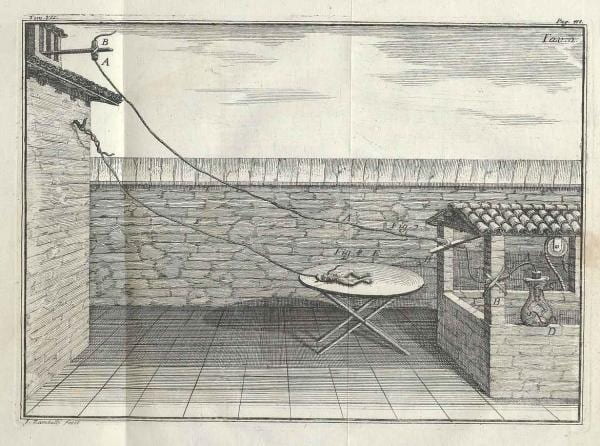
\includegraphics[width=0.6\linewidth]{galvani-experiment_2.jpeg}

\end{figure}
\end{frame}

\begin{frame}{Galvanismo como Espetáculo}

\begin{block}{Fenômeno Social}
\begin{itemize}
\item Demonstrações públicas de galvanismo viraram \textbf{espetáculo}
\item Experimentos com cadáveres sugeriam \textbf{“reanimar” os mortos}
\end{itemize}
\end{block}

\vspace{0.3cm}

\begin{alertblock}{Impacto Cultural}
\centering
Influenciou diretamente: \\[0.2cm]
{\Large \textbf{Frankenstein}}
\end{alertblock}



\end{frame}

\begin{frame}{Galvanismo}
    \begin{figure}
        \centering
        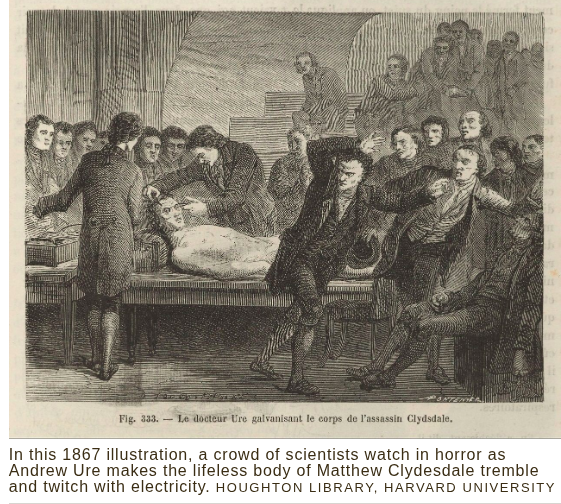
\includegraphics[width=0.5\linewidth]{corpse.png}
    \end{figure}
\end{frame}


\begin{frame}{Densidade de Corrente}
\begin{block}{Definição local}
\[
dI = \mathbf{j} \cdot d\mathbf{S} = \mathbf{j} \cdot \hat{\mathbf{n}}\, dS
\]
\end{block}

\begin{alertblock}{Interpretação}
\begin{itemize}
\item $\mathbf{j}(\mathbf{r},t)$: densidade de corrente
\item Mede o fluxo de carga através de uma superfície
\end{itemize}
\end{alertblock}
\end{frame}

%------------------------------------------------

\begin{frame}{Densidade de Corrente}
    \begin{figure}
        \centering
        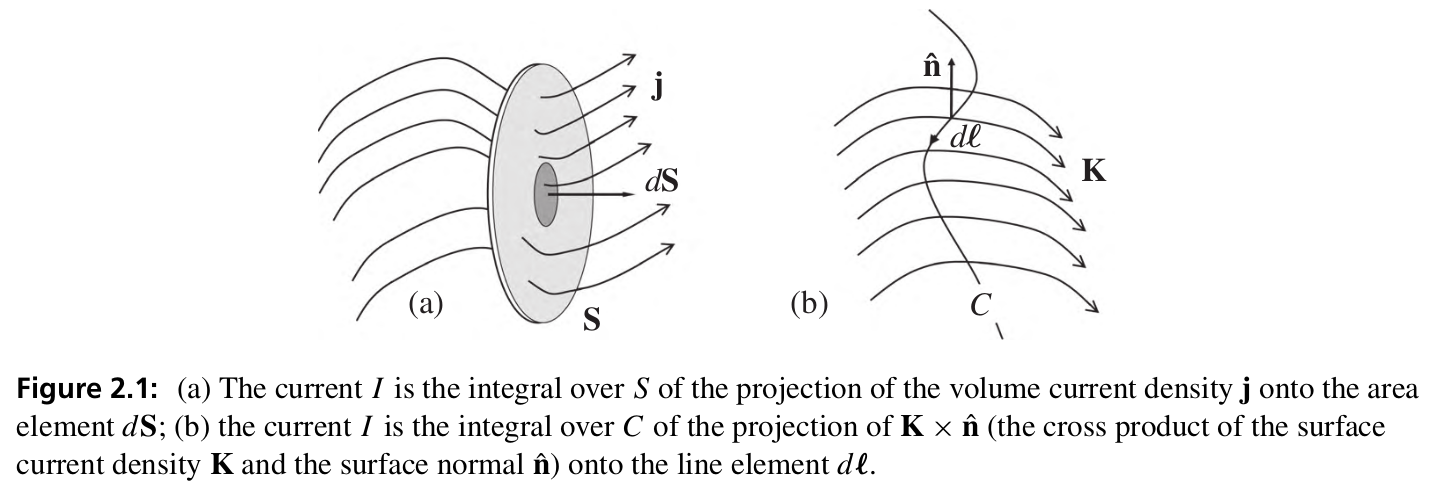
\includegraphics[width=0.9\linewidth]{figure2p1.png}
    \end{figure}
\end{frame}

\begin{frame}{Corrente Total}
\begin{block}{Equação fundamental}
\begin{equation}
I = \frac{dQ}{dt} = \int_S d\mathbf{S} \cdot \mathbf{j}.
\label{eq:2.7}
\tag{2.7}
\end{equation}

\end{block}

\begin{alertblock}{Ideia física}
\begin{itemize}
\item Corrente = fluxo total de carga através da superfície
\end{itemize}
\end{alertblock}
\end{frame}

%------------------------------------------------

\begin{frame}{Corrente como Fluido}
\begin{block}{Relação fundamental}
\begin{equation}
\mathbf{j} = \rho \mathbf{v}.
\label{eq:2.8}
\tag{2.8}
\end{equation}

\end{block}

\begin{alertblock}{Interpretação}
\begin{itemize}
\item $\rho$: densidade de carga
\item $\mathbf{v}$: velocidade do fluxo
\end{itemize}
\end{alertblock}
\end{frame}

%------------------------------------------------

\begin{frame}{Corrente em Superfícies}

Se a carga estiver totalmente confinada a uma superfície bidimensional, é apropriado substituir (2.8) por uma densidade de corrente superficial.

\begin{block}{Densidade superficial}
\begin{equation}
\mathbf{K} = \sigma \mathbf{v}.
\label{eq:2.9}
\tag{2.9}
\end{equation}
\end{block}

\begin{alertblock}{Quando usar}
\begin{itemize}
\item Cargas confinadas a uma superfície (ex: condutores finos)
\end{itemize}
\end{alertblock}
\end{frame}

%------------------------------------------------

\begin{frame}{Corrente ao longo de uma curva}
\begin{block}{Expressão geral}
\begin{equation}
I = \int_C d\boldsymbol{\ell} \cdot (\mathbf{K} \times \hat{\mathbf{n}}) 
= \int_C \mathbf{K} \cdot (\hat{\mathbf{n}} \times d\boldsymbol{\ell}).
\label{eq:2.10}
\end{equation}
(2.10)
\end{block}

\begin{alertblock}{Insight}
\begin{itemize}
\item Apenas a componente de $\mathbf{K}$ normal à curva contribui
\end{itemize}
\end{alertblock}
\notas{pag 1}
\end{frame}


\begin{frame}{Conservação de Carga}

\begin{block}{Princípio fundamental}
A carga elétrica é \textbf{absolutamente conservada} em todos os processos físicos conhecidos.
\end{block}

\vspace{0.2cm}

\begin{block}{Consequência direta}
\begin{itemize}
\item A carga em um volume só muda se houver \textbf{fluxo de partículas carregadas}
\item Entrando ou saindo do volume
\end{itemize}
\end{block}

\vspace{0.2cm}

\begin{alertblock}{Mesmo em processos complexos}
\begin{itemize}
\item Reações químicas criam/destroem espécies
\item Processos quânticos criam/destroem partículas
\end{itemize}

\centering
\textbf{Mas a carga total permanece constante}
\end{alertblock}



\end{frame}
%------------------------------------------------

\begin{frame}{Conservação de Carga — Teste Extremo}

\begin{block}{Ideia do teste}
Se a carga elétrica \textbf{não fosse conservada}, o elétron poderia decair em partículas neutras:
\[
e^- \;\rightarrow\; \text{fótons, neutrinos, etc.}
\]
\end{block}

\vspace{0.3cm}

\begin{alertblock}{Por que isso é importante?}
\begin{itemize}
\item O elétron tem carga $-e$
\item As partículas finais seriam \textbf{neutras}
\item Isso violaria diretamente a \textbf{conservação da carga}
\end{itemize}
\end{alertblock}

\end{frame}

\begin{frame}

\begin{block}{Resultado experimental}
\[
\tau_e > 10^{24}\ \text{anos}
\]

\begin{itemize}
\item Nenhum decaimento observado
\item O elétron é \textbf{extremamente estável}
\end{itemize}
\end{block}

\vspace{0.3cm}

\begin{alertblock}{Mensagem física}
A conservação da carga é uma das leis mais robustas da natureza.
\end{alertblock}

\end{frame}
%------------------------------------------------

\begin{frame}{Forma Integral}
\begin{block}{Aplicando teorema da divergência}
\begin{equation}
I = \int_V d^3 r \, \nabla \cdot \mathbf{j}.
\label{eq:2.11}
\end{equation}
(2.11)
\end{block}

\begin{alertblock}{Significado}
\begin{itemize}
\item Fluxo pela superfície = divergência no volume
\end{itemize}
\end{alertblock}
\end{frame}

%------------------------------------------------

\begin{frame}{Variação da carga}
\begin{block}{Expressão}
\begin{equation}
-\frac{dQ}{dt} = -\frac{d}{dt} \int_V d^3 r \, \rho 
= - \int_V d^3 r \, \frac{\partial \rho}{\partial t}.
\label{eq:2.12}
\end{equation}
(2.12)
\end{block}

\begin{alertblock}{Interpretação}
\begin{itemize}
\item Variação da carga no volume
\end{itemize}
\end{alertblock}
\notas{pag 2}
\end{frame}

%------------------------------------------------

\begin{frame}{Equação da Continuidade}
\begin{block}{Forma local}
\begin{equation}
\frac{\partial \rho}{\partial t} + \nabla \cdot \mathbf{j} = 0.
\label{eq:2.13}
\end{equation}
(2.13)
\end{block}

\begin{alertblock}{Mensagem central}
\begin{itemize}
\item Conservação local da carga
\end{itemize}
\end{alertblock}
\notas{pag 3}
\end{frame}

%------------------------------------------------

\begin{frame}{Cargas Pontuais em Movimento}
\begin{block}{Densidade de carga}
\begin{equation}
\rho(\mathbf{r},t) = \sum_{k=1}^N q_k \delta(\mathbf{r} - \mathbf{r}_k(t)).
\label{eq:2.14}
\end{equation}
(2.14)
\end{block}

\begin{block}{Resultado final para corrente}
\begin{equation}
\mathbf{j}(\mathbf{r},t) = \sum_{k=1}^N q_k \mathbf{v}_k \delta(\mathbf{r} - \mathbf{r}_k).
\label{eq:2.17}
\end{equation}
(2.17)
\end{block}
\notas{pag 3-6}
\end{frame}

%------------------------------------------------
\begin{frame}{2.1.3 Conservação de Carga}

\begin{block}{Princípio fundamental}
\begin{itemize}
\item A carga elétrica é \textbf{absolutamente conservada}
\item Só pode variar em um volume por fluxo através da superfície
\end{itemize}
\end{block}

\begin{alertblock}{Importância}
\begin{itemize}
\item Base de toda a eletrodinâmica
\item Conecta fenômenos clássicos e quânticos
\end{itemize}
\end{alertblock}

\end{frame}

%------------------------------------------------
\begin{frame}{Forma Integral da Corrente}

\begin{block}{Corrente como divergência}
\begin{equation}
I = \int_V d^3 r \, \nabla \cdot \mathbf{j}.
\label{eq:2.11}
\tag{2.11}
\end{equation}
\end{block}

\begin{alertblock}{Interpretação}
\begin{itemize}
\item Fluxo de corrente através da superfície
\item Equivalente à divergência no volume
\end{itemize}
\end{alertblock}

\end{frame}

%------------------------------------------------
\begin{frame}{Variação da Carga no Volume}

\begin{block}{Expressão}
\begin{equation}
-\frac{dQ}{dt} 
= -\frac{d}{dt} \int_V d^3 r \, \rho 
= - \int_V d^3 r \, \frac{\partial \rho}{\partial t}.
\label{eq:2.12}
\tag{2.12}
\end{equation}
\end{block}

\begin{alertblock}{Significado}
\begin{itemize}
\item Variação da carga dentro do volume
\item Relaciona densidade de carga e tempo
\end{itemize}
\end{alertblock}

\end{frame}

%------------------------------------------------
\begin{frame}{Equação da Continuidade}

\begin{block}{Forma local}
\begin{equation}
\frac{\partial \rho}{\partial t} + \nabla \cdot \mathbf{j} = 0.
\label{eq:2.13}
\tag{2.13}
\end{equation}
\end{block}

\begin{alertblock}{Mensagem-chave}
\begin{itemize}
\item Conservação local da carga
\item Sem fontes ou sumidouros de carga
\end{itemize}
\end{alertblock}

\end{frame}

%------------------------------------------------
\begin{frame}{Cargas Pontuais em Movimento}

\begin{block}{Densidade de carga}
\begin{equation}
\rho(\mathbf{r},t) = \sum_{k=1}^{N} q_k \delta(\mathbf{r} - \mathbf{r}_k(t)).
\label{eq:2.14}
\tag{2.14}
\end{equation}
\end{block}

\begin{alertblock}{Interpretação}
\begin{itemize}
\item Soma de contribuições localizadas
\item Cada carga descrita por uma delta de Dirac
\end{itemize}
\end{alertblock}

\end{frame}

%------------------------------------------------
\begin{frame}{Derivação da Corrente}

\begin{block}{Evolução temporal}
\begin{equation}
\frac{\partial \rho}{\partial t}
= \sum_k q_k \frac{\partial}{\partial t} \delta(\mathbf{r}-\mathbf{r}_k)
= - \sum_k q_k \mathbf{v}_k \cdot \nabla \delta(\mathbf{r}-\mathbf{r}_k).
\label{eq:2.15}
\tag{2.15}
\end{equation}
\end{block}

\begin{block}{Forma equivalente}
\begin{equation}
\frac{\partial \rho}{\partial t}
= - \nabla \cdot \sum_k q_k \mathbf{v}_k \delta(\mathbf{r}-\mathbf{r}_k).
\label{eq:2.16}
\tag{2.16}
\end{equation}
\end{block}

\begin{block}{Densidade de corrente}
\begin{equation}
\mathbf{j}(\mathbf{r},t)
= \sum_{k=1}^{N} q_k \mathbf{v}_k \delta(\mathbf{r}-\mathbf{r}_k).
\label{eq:2.17}
\tag{2.17}
\end{equation}
\end{block}
\notas{pag 4-5}
\end{frame}

%------------------------------------------------
\begin{frame}{2.2 Equações de Maxwell no Vácuo}

\begin{block}{Unificação}
\begin{itemize}
\item<1-> Eletricidade, magnetismo e óptica apareciam como áreas separadas
\item<2-> \textbf{Maxwell} mostrou que todas fazem parte de uma mesma teoria
\item<3-> Essa unificação foi apresentada no \emph{Treatise on Electricity and Magnetism} (1873)
\end{itemize}
\end{block}

\begin{alertblock}{Impacto conceitual}<4->
A interação eletromagnética não é um conjunto de leis isoladas, mas uma
\textbf{estrutura matemática unificada baseada em campos}.
\end{alertblock}

\end{frame}

%------------------------------------------------
\begin{frame}{Da descrição experimental à teoria}

\begin{block}{Leitura histórica}
\begin{itemize}
\item<1-> Maxwell partiu de muitos resultados experimentais dispersos
\item<2-> Seu objetivo era \textbf{matematizar} os fenômenos elétricos e magnéticos
\item<3-> Uma geração depois, Hertz resumiu isso dizendo:
\end{itemize}
\end{block}

\begin{alertblock}<4->
\centering
\emph{“Maxwell’s theory is Maxwell’s system of equations.”}
\end{alertblock}

\begin{block}{Observação}<5->
A formulação moderna em \textbf{quatro equações} é uma versão condensada da formulação original.
\end{block}

\end{frame}

%------------------------------------------------
\begin{frame}{2.2.1 Eletrostática}

\begin{block}{Lei de Coulomb}
Trabalhos experimentais de Priestley, Cavendish e Coulomb, no final do século XVIII, estabeleceram a natureza da força entre objetos carregados em repouso. Extrapolando para o caso de cargas puntuais, a força sobre uma carga $q$ no ponto $\mathbf{r}$ devido a $N$ cargas puntuais $q_k$ nos pontos $\mathbf{r}_k$ é dada pela lei do inverso do quadrado de Coulomb.
\begin{equation}
\mathbf{F} = \frac{1}{4\pi\epsilon_0} \sum_{k=1}^N q q_k
\frac{\mathbf{r}-\mathbf{r}_k}{|\mathbf{r}-\mathbf{r}_k|^3}
\tag{2.18}
\end{equation}
\end{block}

\begin{itemize}
\item<2-> A força entre cargas puntuais segue uma lei de \textbf{inverso do quadrado}
\item<3-> A direção da força é dada pela reta que liga fonte e observador
\item<4-> A superposição já aparece implicitamente na soma sobre \(k\)
\end{itemize}

\begin{alertblock}{Impacto conceitual}<5->
A eletrostática começa como uma teoria de \textbf{forças entre cargas}.
\end{alertblock}
\notas{pag 6}
\end{frame}

%------------------------------------------------
\begin{frame}{Da força ao campo elétrico}

\begin{block}{Definição de campo}
\begin{equation}
\mathbf{F} = q\,\mathbf{E}(\mathbf{r})
\tag{2.19}
\end{equation}
\end{block}

\begin{itemize}
\item<2-> Em vez de pensar diretamente em força entre duas cargas...
\item<3-> ...passamos a descrever um \textbf{campo} presente no espaço
\item<4-> A partícula de prova apenas responde ao valor local de \(\mathbf{E}\)
\end{itemize}

\begin{alertblock}{Impacto conceitual}<5->
A pergunta deixa de ser “qual carga puxa qual?” e passa a ser:
\[
\textit{qual é o campo neste ponto do espaço?}
\]
\end{alertblock}

\end{frame}

%------------------------------------------------
\begin{frame}{Campo elétrico de uma distribuição}

\begin{equation}
\mathbf{E}(\mathbf{r}) = \frac{1}{4\pi\epsilon_0}
\int d^3r' \, \rho(\mathbf{r}')
\frac{\mathbf{r}-\mathbf{r}'}{|\mathbf{r}-\mathbf{r}'|^3}
\tag{2.20}
\end{equation}

\begin{itemize}
\item<2-> Cada elemento \(d^3r'\) contribui para o campo em \(\mathbf r\)
\item<3-> O campo total é a soma vetorial de todas essas contribuições
\end{itemize}

\begin{alertblock}{Princípio de superposição}<4->
O campo produzido por uma distribuição arbitrária de carga é a soma dos campos
produzidos por cada uma de suas partes constituintes.
\end{alertblock}

\end{frame}

%------------------------------------------------
\begin{frame}{As identidades matemáticas essenciais}

\begin{block}{Ferramentas}
\begin{equation}
\nabla \frac{1}{|\mathbf{r}-\mathbf{r}'|}
=
-\frac{\mathbf{r}-\mathbf{r}'}{|\mathbf{r}-\mathbf{r}'|^3}
\end{equation}

\begin{equation}
\nabla^2 \frac{1}{|\mathbf{r}-\mathbf{r}'|}
=
-4\pi \delta(\mathbf{r}-\mathbf{r}')
\tag{2.21}
\end{equation}
\end{block}

\begin{itemize}
\item<2-> A primeira relaciona o potencial coulombiano ao campo
\item<3-> A segunda conecta o potencial a uma \textbf{fonte localizada}
\end{itemize}

\begin{alertblock}{Ideia}<4->
Essas identidades permitem passar da forma integral para a forma local das equações.
\end{alertblock}
\notas{pag 7}
\end{frame}

%------------------------------------------------
\begin{frame}{Equações da eletrostática}

\begin{equation}
\nabla \cdot \mathbf{E} = \frac{\rho}{\epsilon_0}
\end{equation}

\begin{equation}
\nabla \times \mathbf{E} = 0
\tag{2.22}
\end{equation}

\begin{itemize}
\item<2-> A divergência liga o campo elétrico à densidade de carga
\item<3-> O rotacional nulo mostra que, em eletrostática, \(\mathbf E\) é irrotacional
\end{itemize}

\begin{alertblock}{Impacto conceitual}<4->
A primeira é a \textbf{Lei de Gauss} e já tem a cara da teoria de campos:
\[
\text{fontes locais} \longrightarrow \text{estrutura local do campo}
\]
\end{alertblock}
\notas{pag 7-8}
\end{frame}


\begin{frame}{Ideia central}
\begin{block}{Objetivo}
Mostrar como as identidades
\[
\nabla \frac{1}{|\mathbf{r}-\mathbf{r}'|}
\quad \text{e} \quad
\nabla^2 \frac{1}{|\mathbf{r}-\mathbf{r}'|}
\]
permitem passar da forma \textbf{integral} para a forma \textbf{local}.
\end{block}
\end{frame}

%--------------------------------------------------

\begin{frame}{Potencial eletrostático (forma integral)}
\begin{block}{Definição}
\begin{equation}
\phi(\mathbf{r}) =
\frac{1}{4\pi\epsilon_0}
\int \frac{\rho(\mathbf{r}')}{|\mathbf{r}-\mathbf{r}'|} \, d^3 r'
\label{eq:potencial_integral}
\end{equation}
\end{block}

\begin{itemize}
\item Cada elemento de carga contribui com um potencial coulombiano.
\item A informação da fonte está distribuída na integral.
\end{itemize}
\end{frame}

%--------------------------------------------------

\begin{frame}{Campo elétrico a partir do potencial}
\begin{block}{Relação fundamental}
\begin{equation}
\mathbf{E}(\mathbf{r}) = -\nabla \phi(\mathbf{r})
\label{eq:E_grad_phi}
\end{equation}
\end{block}

Aplicando o gradiente em \eqref{eq:potencial_integral}:

\begin{equation}
\mathbf{E}(\mathbf{r}) =
-\frac{1}{4\pi\epsilon_0}
\int \rho(\mathbf{r}')
\nabla \left( \frac{1}{|\mathbf{r}-\mathbf{r}'|} \right)
\, d^3 r'
\end{equation}

\end{frame}

%--------------------------------------------------

\begin{frame}{Uso da identidade do gradiente}
\begin{block}{Identidade chave}
\begin{equation}
\nabla \frac{1}{|\mathbf{r}-\mathbf{r}'|}
=
-\frac{\mathbf{r}-\mathbf{r}'}{|\mathbf{r}-\mathbf{r}'|^3}
\label{eq:grad_green}
\end{equation}
\end{block}

Substituindo:

\begin{equation}
\mathbf{E}(\mathbf{r}) =
\frac{1}{4\pi\epsilon_0}
\int \rho(\mathbf{r}')
\frac{\mathbf{r}-\mathbf{r}'}{|\mathbf{r}-\mathbf{r}'|^3}
\, d^3 r'
\end{equation}

\begin{alertblock}{Interpretação}
Obtivemos o campo elétrico como superposição das contribuições de Coulomb.
\end{alertblock}

\end{frame}

%--------------------------------------------------

\begin{frame}{Agora: da forma integral para a forma local}
Queremos obter uma equação diferencial para \(\phi\).

Aplicamos o Laplaciano em \eqref{eq:potencial_integral}:

\begin{equation}
\nabla^2 \phi(\mathbf{r}) =
\frac{1}{4\pi\epsilon_0}
\int \rho(\mathbf{r}')
\nabla^2 \left( \frac{1}{|\mathbf{r}-\mathbf{r}'|} \right)
\, d^3 r'
\end{equation}

\end{frame}

%--------------------------------------------------

\begin{frame}{Uso da identidade com delta de Dirac}
\begin{block}{Identidade fundamental}
\begin{equation}
\nabla^2 \frac{1}{|\mathbf{r}-\mathbf{r}'|}
=
-4\pi \delta(\mathbf{r}-\mathbf{r}')
\label{eq:lap_green}
\end{equation}
\end{block}

Substituindo:

\begin{equation}
\nabla^2 \phi(\mathbf{r}) =
-\frac{1}{\epsilon_0}
\int \rho(\mathbf{r}')
\delta(\mathbf{r}-\mathbf{r}')
\, d^3 r'
\end{equation}

\end{frame}

%--------------------------------------------------

\begin{frame}{Colapso da integral}
\begin{block}{Propriedade da delta}
\begin{equation}
\int f(\mathbf{r}') \delta(\mathbf{r}-\mathbf{r}') d^3 r'
= f(\mathbf{r})
\end{equation}
\end{block}

Aplicando:

\begin{equation}
\nabla^2 \phi(\mathbf{r}) =
-\frac{\rho(\mathbf{r})}{\epsilon_0}
\label{eq:poisson}
\end{equation}

\begin{alertblock}{Resultado}
Obtivemos a \textbf{equação de Poisson} (forma local).
\end{alertblock}

\end{frame}

%--------------------------------------------------

\begin{frame}{Equações locais da eletrostática}
Usando \(\mathbf{E} = -\nabla \phi\):

\begin{equation}
\nabla \cdot \mathbf{E} = \frac{\rho}{\epsilon_0}
\end{equation}

\begin{equation}
\nabla \times \mathbf{E} = 0
\end{equation}

\begin{block}{Conclusão}
As identidades com \(1/|\mathbf{r}-\mathbf{r}'|\) permitem:
\begin{itemize}
\item Ir da descrição global (integral)
\item Para uma descrição local (equações diferenciais)
\end{itemize}
\end{block}

\end{frame}

\begin{frame}{Cuidado! (Eletrostática)}

\begin{block}{Hipótese}
Na eletrostática:
\begin{equation}
\mathbf{E} = -\nabla \phi
\end{equation}
\end{block}

\begin{block}{Demonstração}
\begin{align}
\nabla \times \mathbf{E}
&= \nabla \times (-\nabla \phi) \\
&= - \nabla \times (\nabla \phi) \\
&= 0
\end{align}
\end{block}

\begin{alertblock}{Conclusão}
\begin{equation}
\nabla \times \mathbf{E} = 0
\end{equation}
\end{alertblock}

\end{frame}

%--------------------------------------------------

\begin{frame}{Cuidado! (Não eletrostático)}

\begin{alertblock}{Quando isso deixa de valer}
Se o campo magnético varia no tempo:
\begin{equation}
\nabla \times \mathbf{E} = -\frac{\partial \mathbf{B}}{\partial t}
\end{equation}
\end{alertblock}

\begin{itemize}
\item O campo elétrico deixa de ser conservativo
\item Linhas de campo podem formar circuitos fechados
\item Não é possível escrever apenas \(\mathbf{E} = -\nabla \phi\)
\end{itemize}

\vspace{0.3cm}

\begin{block}{Forma geral}
\begin{equation}
\mathbf{E} = -\nabla \phi - \frac{\partial \mathbf{A}}{\partial t}
\end{equation}
\end{block}

\end{frame}

%------------------------------------------------
\begin{frame}{2.2.2 O conceito de campo}

\begin{block}{Mudança de paradigma}
\begin{itemize}
\item<1-> Antes: ação à distância entre cargas
\item<2-> Depois: campos preenchendo todo o espaço
\item<3-> A força passa a ser mediada pelo valor local do campo
\end{itemize}
\end{block}

\begin{alertblock}{Mensagem física}<4->
Para problemas estáticos, as duas visões são equivalentes.

\vspace{0.1cm}
Mas a visão de campo se torna \textbf{muito superior} quando passamos a fenômenos dependentes do tempo.
\end{alertblock}

\end{frame}

%------------------------------------------------
\begin{frame}{Campos como entidades físicas}

\begin{itemize}
\item<1-> O campo não é apenas um artifício matemático
\item<2-> Ele pode possuir:
\begin{itemize}
\item<2-> energia
\item<2-> momento linear
\item<2-> momento angular
\end{itemize}
\item<3-> Pode existir e evoluir dinamicamente
\end{itemize}

\begin{alertblock}{Impacto conceitual}<4->
Campos têm o mesmo status mecânico que partículas:
\[
\textbf{campos são objetos físicos reais}
\]
\end{alertblock}

\end{frame}

%------------------------------------------------
\begin{frame}{2.2.3 Magnetostática}

\begin{block}{Linha histórica}
\begin{itemize}
\item<1-> Gilbert: a Terra se comporta como um ímã gigante
\item<2-> Michell, Coulomb e Gauss: força entre polos magnéticos
\item<3-> Oersted (1820): corrente elétrica produz efeitos magnéticos
\end{itemize}
\end{block}

\begin{alertblock}{Mensagem-chave}<4->
A magnetostática mostra que \textbf{correntes} desempenham para o campo magnético
um papel análogo ao das \textbf{cargas} para o campo elétrico.
\end{alertblock}

\end{frame}

%------------------------------------------------
\begin{frame}{Força entre correntes}

\begin{equation}
\mathbf{F} =
-\frac{\mu_0}{4\pi}
\oint I\, d\boldsymbol{\ell}
\cdot
\sum_k
\oint I_k\, d\boldsymbol{\ell}_k\,
\frac{\mathbf{r}-\mathbf{r}_k}{|\mathbf{r}-\mathbf{r}_k|^3}
\tag{2.23}
\end{equation}

\begin{figure}
    \centering
    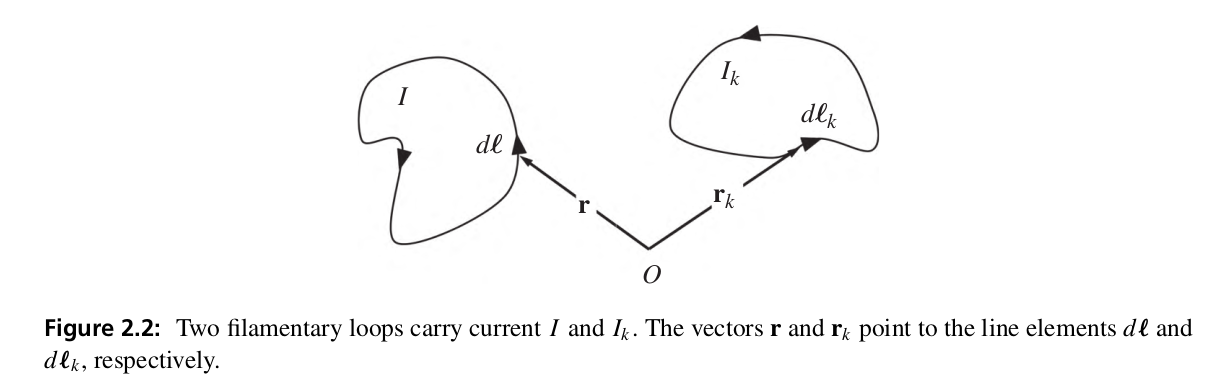
\includegraphics[width=0.8\linewidth]{correntes.png}

\end{figure}

\end{frame}


\begin{frame}{Força entre correntes}

\begin{equation}
\mathbf{F} =
-\frac{\mu_0}{4\pi}
\oint I\, d\boldsymbol{\ell}
\cdot
\sum_k
\oint I_k\, d\boldsymbol{\ell}_k\,
\frac{\mathbf{r}-\mathbf{r}_k}{|\mathbf{r}-\mathbf{r}_k|^3}
\tag{2.23}
\end{equation}
\begin{itemize}
\item<2-> Ampère descreve a força sobre um circuito devido a outros circuitos
\item<3-> A estrutura lembra a de Coulomb, mas agora para elementos de corrente
\end{itemize}

\begin{alertblock}{Leitura conceitual}<4->
A magnetostática também pode começar como uma teoria de \textbf{forças},
mas naturalmente conduz ao conceito de campo magnético.
\end{alertblock}

\end{frame}

%------------------------------------------------
\begin{frame}{Definição operacional de campo magnético}

\begin{equation}
\mathbf{F} = \oint I\, d\boldsymbol{\ell} \times \mathbf{B}(\mathbf{r})
\tag{2.24}
\end{equation}

\begin{itemize}
\item<2-> Assim como \(\mathbf F = q\mathbf E\) definiu o campo elétrico...
\item<3-> ...essa expressão define o campo magnético pela força sobre um circuito
\end{itemize}

\begin{alertblock}{Impacto conceitual}<4->
\(\mathbf E\) e \(\mathbf B\) surgem de maneira paralela:
um pela força sobre cargas, outro pela força sobre correntes.
\end{alertblock}

\end{frame}

%------------------------------------------------
\begin{frame}{Lei de Biot--Savart}

\begin{equation}
\mathbf{B}(\mathbf{r}) =
\frac{\mu_0}{4\pi}
\sum_k \oint I_k\, d\boldsymbol{\ell}_k
\times
\frac{\mathbf{r}-\mathbf{r}_k}{|\mathbf{r}-\mathbf{r}_k|^3}
\tag{2.25}
\end{equation}

\begin{itemize}
\item<2-> Cada elemento de corrente contribui para \(\mathbf B(\mathbf r)\)
\item<3-> O campo total é novamente obtido por \textbf{superposição}
\end{itemize}

\begin{alertblock}{Comparação}<4->
Biot--Savart para \(\mathbf B\) ocupa, na magnetostática,
o papel que a integral coulombiana ocupa na eletrostática.
\end{alertblock}

\end{frame}

%------------------------------------------------
\begin{frame}{Forma contínua da magnetostática}

\begin{equation}
\mathbf{B}(\mathbf{r}) =
\frac{\mu_0}{4\pi}
\int d^3r' \,
\mathbf{j}(\mathbf{r}') \times
\frac{\mathbf{r}-\mathbf{r}'}{|\mathbf{r}-\mathbf{r}'|^3}
\tag{2.26}
\end{equation}

\begin{itemize}
\item<2-> Passamos de circuitos filiformes para distribuições contínuas de corrente
\item<3-> A fonte do campo magnético é a densidade de corrente \(\mathbf j\)
\end{itemize}

\begin{alertblock}{Impacto conceitual}<4->
Na linguagem de campos:
\[
\text{cargas } \rho \;\longrightarrow\; \mathbf E,
\qquad
\text{correntes } \mathbf j \;\longrightarrow\; \mathbf B
\]
\end{alertblock}

\end{frame}


%------------------------------------------------
\begin{frame}{Lei de Biot–Savart (forma discreta)}

\begin{block}{Expressão para correntes em fios}
\begin{equation}
\mathbf{B}(\mathbf r)=\frac{\mu_0}{4\pi}\sum_k \oint I_k\, d\boldsymbol{\ell}_k\times
\frac{\mathbf r-\mathbf r_k}{|\mathbf r-\mathbf r_k|^3}
\tag{2.25}
\end{equation}
\end{block}

\begin{itemize}
\item<2-> Soma sobre circuitos \(k\)
\item<3-> Integrais de linha ao longo dos fios
\item<4-> Cada elemento \(I_k d\boldsymbol{\ell}_k\) contribui para o campo
\end{itemize}

\end{frame}

%------------------------------------------------
\begin{frame}{Limitação da descrição}

\begin{block}{Problema}
\begin{itemize}
\item<1-> A expressão assume correntes confinadas a fios
\item<2-> Mas em geral temos correntes distribuídas no volume
\item<3-> Precisamos de uma descrição contínua da corrente
\end{itemize}
\end{block}


\end{frame}

%------------------------------------------------
\begin{frame}{Introduzindo a densidade de corrente}

\begin{block}{Nova variável}
\[
\mathbf j(\mathbf r)
\]
\end{block}

\begin{itemize}
\item<2-> Corrente por unidade de área
\item<3-> Descreve distribuição contínua de carga em movimento
\end{itemize}

\only<4->{
\begin{alertblock}{}
Substituímos a corrente discreta por uma densidade contínua
\end{alertblock}
}

\end{frame}

%------------------------------------------------
\begin{frame}{Substituição fundamental}

\begin{block}{Elemento de corrente}
\[
I\, d\boldsymbol{\ell}
\]
\end{block}

\begin{block}<2->{Equivalente contínuo}
\[
\mathbf j(\mathbf r')\, d^3r'
\]
\end{block}

\begin{itemize}
\item<3-> Volume dividido em tubos de corrente
\item<4-> Em cada tubo:
\[
\mathbf j\,dA = I
\]
\item<5-> Logo:
\[
\mathbf j\,d^3r = I\,d\boldsymbol{\ell}
\]
\end{itemize}

\end{frame}

%------------------------------------------------
\begin{frame}{Da soma à integral}

\begin{block}{Substituição global}
\begin{itemize}
\item<1-> Soma sobre fios:
\[
\sum_k \oint I_k\, d\boldsymbol{\ell}_k
\]
\item<2-> Torna-se:
\[
\int d^3r'\, \mathbf j(\mathbf r')
\]
\end{itemize}
\end{block}

\only<3->{
\begin{alertblock}{}
\centering
\Large \textbf{Fonte discreta $\rightarrow$ variável contínua}

\vspace{0.2cm}

\[
\mathbf r_k \;\rightarrow\; \mathbf r'
\]
\end{alertblock}
}

\end{frame}

%------------------------------------------------
\begin{frame}{Lei de Biot–Savart (forma contínua)}

\begin{equation}
\mathbf{B}(\mathbf r)=\frac{\mu_0}{4\pi}
\int d^3r'\,\mathbf j(\mathbf r')\times
\frac{\mathbf r-\mathbf r'}{|\mathbf r-\mathbf r'|^3}
\tag{2.26}
\end{equation}

\begin{alertblock}{Resultado final}
\begin{itemize}
\item Correntes discretas $\rightarrow$ distribuição contínua
\item Soma de fios $\rightarrow$ integral de volume
\end{itemize}
\end{alertblock}

\begin{block}<2->{Mensagem conceitual}
\centering
\textbf{A fonte do campo magnético é a densidade de corrente}
\end{block}

\end{frame}


\begin{frame}{Equações da Magnetostática}

\begin{block}{Resultado fundamental}
Em 1851, William Thomson (Lord Kelvin) mostrou que o campo magnético gerado por correntes e ímãs permanentes satisfaz:
\end{block}

\vspace{0.2cm}

\begin{equation}
\nabla \cdot \mathbf{B} = 0
\qquad \text{e} \qquad
\nabla \times \mathbf{B} = \mu_0 \mathbf{j}
\tag{2.27}
\end{equation}

\vspace{0.3cm}

\begin{alertblock}{Consistência}
A expressão geral do campo magnético é consistente com essas equações desde que a corrente satisfaça:
\end{alertblock}

\vspace{0.1cm}

\begin{equation}
\nabla \cdot \mathbf{j} = 0
\tag{2.28}
\end{equation}

\end{frame}

\begin{frame}

\begin{block}{Interpretação}
\begin{itemize}
\item $\nabla \cdot \mathbf{B} = 0$ \;\;\; $\rightarrow$ não existem monopolos magnéticos
\item $\nabla \times \mathbf{B} = \mu_0 \mathbf{j}$ \;\;\; $\rightarrow$ correntes geram campo magnético
\end{itemize}
\end{block}

\vspace{0.2cm}

\begin{center}
\small
A segunda equação é válida apenas para correntes estacionárias e é conhecida como \textbf{Lei de Ampère}.
\end{center}

\end{frame}
%------------------------------------------------




\begin{frame}

\begin{alertblock}{Fechamento conceitual}
Em estática, Maxwell já aparece em embrião:

\[
\rho \;\text{gera}\; \mathbf E,
\qquad
\mathbf j \;\text{gera}\; \mathbf B.
\]

O próximo passo será mostrar como, no regime dinâmico, \(\mathbf E\) e \(\mathbf B\) passam a gerar um ao outro.
\end{alertblock}

\end{frame}

{
\setbeamercolor{background canvas}{bg=black}
\begin{frame}[plain]
\centering
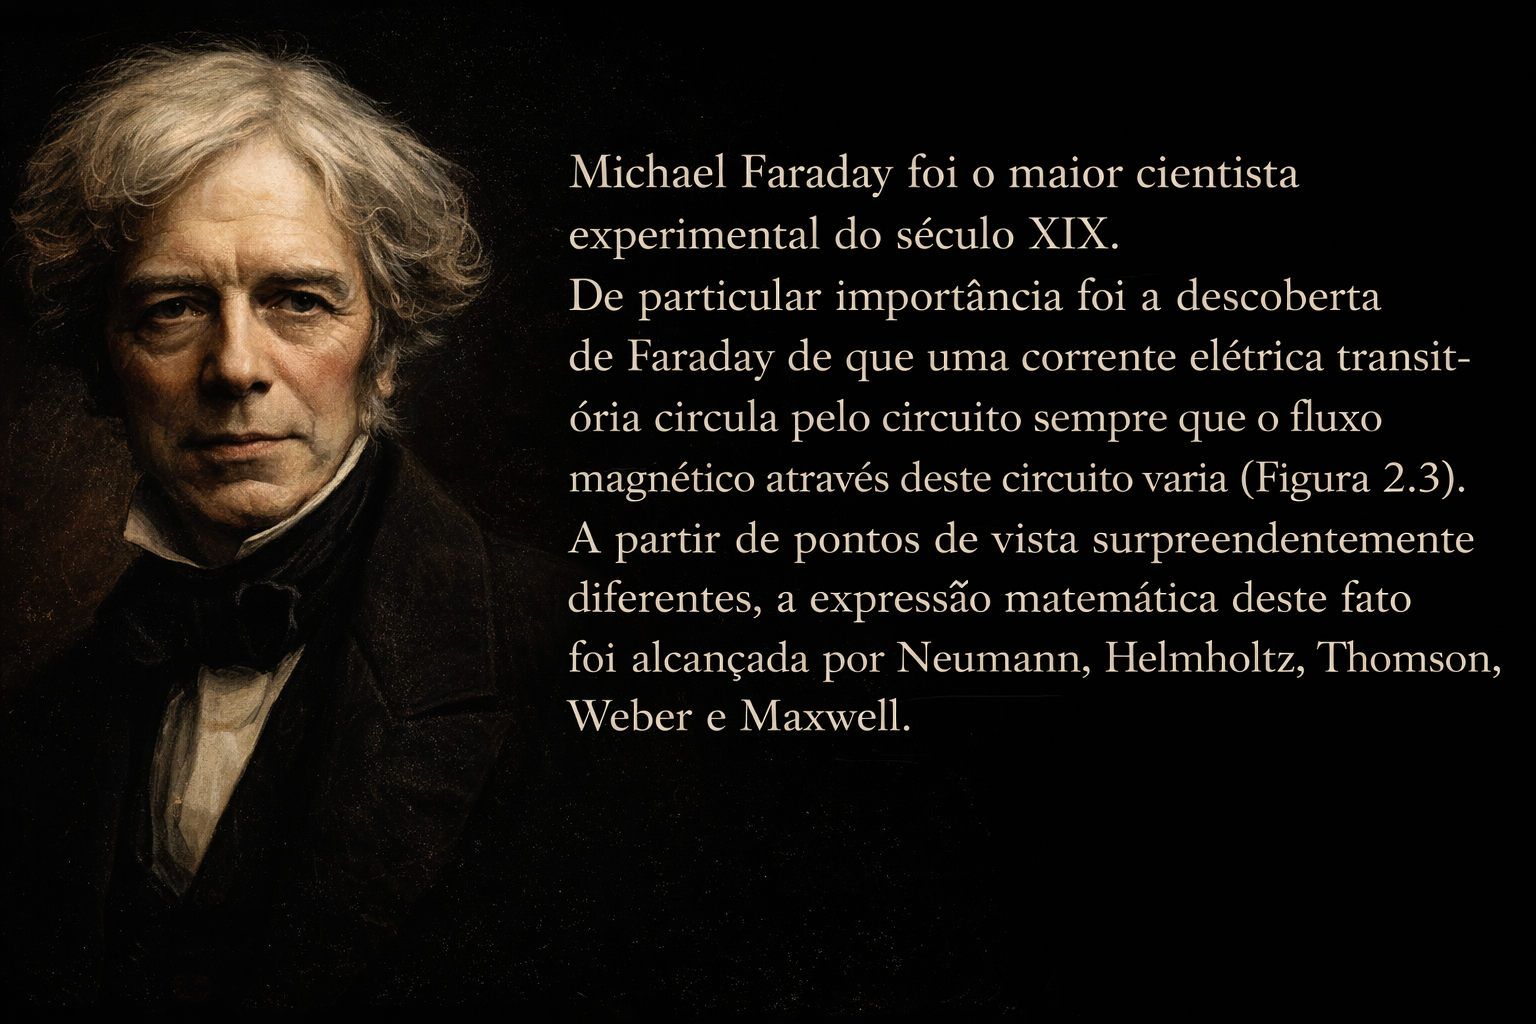
\includegraphics[width=\paperwidth,height=\paperheight,keepaspectratio]{Faraday.png}
\end{frame}
}

\begin{frame}{Experimento de Faraday}

\begin{center}
\only<1>{
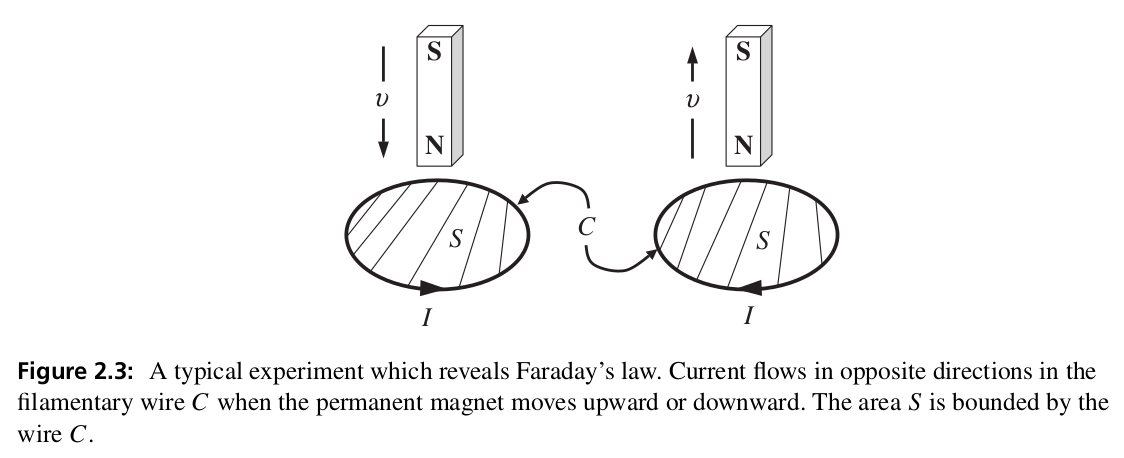
\includegraphics[width=0.9\linewidth]{figure2p3.png}
}
\end{center}

\begin{block}<2->{Observação}
\begin{itemize}
\item Movimento do ímã $\Rightarrow$ corrente no circuito
\item Sentido da corrente depende do movimento
\end{itemize}
\end{block}

\end{frame}
%------------------------------------------------
\begin{frame}{Lei de Faraday}

\begin{block}{Descoberta experimental}
\begin{itemize}
\item<1-> Michael Faraday mostrou que uma corrente elétrica é induzida
\item<2-> Sempre que o \textbf{fluxo magnético varia}
\end{itemize}
\end{block}

\begin{alertblock}<3->
\centering
\textbf{Variação de fluxo magnético $\Rightarrow$ corrente elétrica}
\end{alertblock}

\end{frame}

%------------------------------------------------
\begin{frame}{Expressão matemática}

\begin{block}{Lei de Faraday}
\begin{equation}
-\frac{d}{dt}\int_S \mathbf{B}\cdot d\mathbf{S} = IR
\tag{2.29}
\end{equation}
\end{block}

\begin{itemize}
\item<2-> Lado esquerdo: variação do fluxo magnético
\item<3-> Lado direito: corrente no circuito
\end{itemize}


\begin{alertblock}<4->
\centering
\textbf{O campo magnético variável gera corrente elétrica}
\end{alertblock}


\notas{Analise dimensional pag 9}
\end{frame}

%------------------------------------------------
\begin{frame}{Interpretação física}

\begin{block}{Geometria}
\begin{itemize}
\item<1-> \(S\): superfície limitada pelo circuito \(C\)
\item<2-> \(d\mathbf{S}\): orientação dada pela regra da mão direita
\end{itemize}
\end{block}

\only<3->{
\begin{alertblock}{Lei de Lenz}
O sinal negativo expressa que a corrente induzida se opõe à variação do fluxo magnético.
\end{alertblock}
}

\only<4->{
\begin{itemize}
\item A corrente induzida cria um campo magnético que resiste à mudança do fluxo original.
\end{itemize}
}

\end{frame}

%------------------------------------------------


%------------------------------------------------
\begin{frame}{Da forma integral à diferencial}

\begin{block}{Lei de Ohm}
\begin{equation}
IR = \oint_C \mathbf{E}\cdot d\boldsymbol{\ell}
\tag{2.30}
\end{equation}
\end{block}

\begin{itemize}
\item<2-> Substituímos em (2.29)
\item<3-> Aplicamos o teorema de Stokes
\end{itemize}

\begin{block}<4->{Resultado final}
\begin{equation}
\nabla \times \mathbf{E} = -\frac{\partial \mathbf{B}}{\partial t}
\tag{2.31}
\end{equation}
\end{block}


\only<5->{
\begin{itemize}
\item Terceira equação de Maxwell
\end{itemize}
}

\notas{Notas: pag 10}
\end{frame}

% =========================================================
% 2.2.5 The Displacement Current
% =========================================================

\section{2.2 Fontes e equações de Maxwell}
\subsection{2.2.5 Corrente de Deslocamento}

\begin{frame}{2.2.5 Corrente de Deslocamento}
\begin{block}{Ideia central}
A \textbf{corrente de deslocamento} foi a contribuição conceitual decisiva de Maxwell para fechar a estrutura do eletromagnetismo.  
Ao perceber que a lei de Ampère, na forma original, falhava em situações com \textbf{campos elétricos variando no tempo}, Maxwell introduziu um novo termo efetivo associado a
\[
\frac{\partial \mathbf{E}}{\partial t}.
\]
\end{block}

\vspace{0.3cm}

\begin{itemize}
\item A densidade de corrente de condução \(\mathbf{j}\) não é suficiente em todos os casos.
\item É necessário acrescentar uma contribuição proporcional à variação temporal do campo elétrico.
\item Isso conduz à forma final da lei de Ampère-Maxwell.
\end{itemize}
\end{frame}

\begin{frame}{2.2.5 Corrente de Deslocamento}
\begin{alertblock}{Corrente de deslocamento}
Define-se a corrente de deslocamento por
\[
\mathbf{j}_D=\epsilon_0\,\frac{\partial \mathbf{E}}{\partial t}.
\]
\end{alertblock}

\vspace{0.2cm}

Substituindo esse termo na lei de Ampère, obtém-se a quarta e última equação de Maxwell:

\begin{equation}
\nabla\times\mathbf{B}
=
\mu_0\,\mathbf{j}
+
\frac{1}{c^2}\frac{\partial \mathbf{E}}{\partial t}.
\tag{2.32}
\label{eq:ampere-maxwell-232}
\end{equation}

\begin{block}{Leitura física}
Mesmo na ausência de corrente material atravessando uma região, uma variação temporal de \(\mathbf{E}\) também atua como \textbf{fonte de campo magnético}.
\end{block}
\end{frame}

\begin{frame}{2.2.5 Corrente de Deslocamento}
\begin{columns}[T,onlytextwidth]
\column{0.56\textwidth}
\begin{block}{Consistência teórica}
Hoje é comum dizer que a corrente de deslocamento é \textbf{necessária} para compatibilizar:
\begin{itemize}
\item a lei de Ampère-Maxwell;
\item a lei de Gauss;
\item a equação da continuidade.
\end{itemize}
\end{block}

\vspace{0.2cm}

\begin{itemize}
\item Sem esse termo, a conservação de carga não se encaixa de forma consistente no conjunto das equações.
\item Historicamente, Maxwell chegou a esse termo antes da formulação moderna baseada em conservação de carga.
\end{itemize}

\column{0.40\textwidth}
\begin{block}{Nota histórica}
Em seus trabalhos iniciais, Maxwell utilizou um \textbf{modelo mecânico} de vórtices e esferas intermediárias para inferir a existência dessa nova corrente.
\end{block}
\end{columns}
\end{frame}

\begin{frame}{2.2.5 Corrente de Deslocamento: modelo mecânico de Maxwell}

\begin{figure}
    \centering
    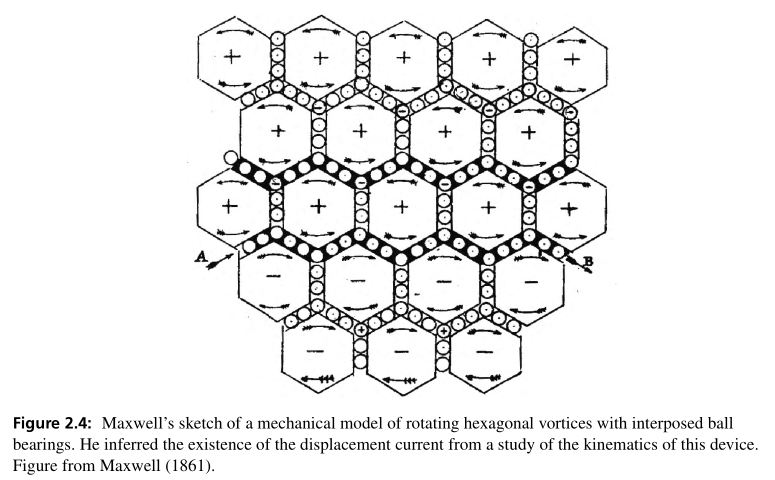
\includegraphics[width=0.5\linewidth]{fig2p4.png}
\end{figure}

\vspace{0.15cm}

\begin{block}{Mensagem física}
A intuição de Maxwell era que a estrutura interna do meio eletromagnético deveria permitir uma transmissão contínua do efeito mesmo onde não houvesse corrente de condução.
\end{block}
\end{frame}


% =========================================================
% Prova: Corrente de deslocamento e consistência
% =========================================================

\begin{frame}{Consistência entre Ampère, Gauss e continuidade}
\small

\begin{block}{Problema}
Queremos verificar se a lei de Ampère é consistente com:
\begin{itemize}\setlength{\itemsep}{2pt}
\item a lei de Gauss;
\item a equação da continuidade.
\end{itemize}
\end{block}

\vspace{0.1cm}

\begin{equation}
\nabla\times \mathbf{B}=\mu_0 \mathbf{j}
\tag{2.30}
\label{eq:ampere_old}
\end{equation}

\begin{equation}
\nabla\cdot \mathbf{E}=\frac{\rho}{\epsilon_0}
\tag{2.31}
\label{eq:gauss}
\end{equation}

\begin{equation}
\frac{\partial \rho}{\partial t}+\nabla\cdot \mathbf{j}=0
\tag{2.13}
\label{eq:continuity}
\end{equation}

\end{frame}


\begin{frame}{Inconsistência da lei de Ampère original}
\small

Tomando a divergência da lei de Ampère:

\begin{equation}
\nabla\cdot(\nabla\times \mathbf{B})
=
\mu_0 \nabla\cdot \mathbf{j}
\label{eq:div_ampere_old}
\end{equation}

Mas sabemos que:

\begin{equation}
\nabla\cdot(\nabla\times \mathbf{B})=0
\label{eq:div_curl}
\end{equation}

Logo,

\begin{equation}
\nabla\cdot \mathbf{j}=0
\label{eq:wrong_result}
\end{equation}

\vspace{0.1cm}

\begin{alertblock}{Problema}
Isso implica \(\partial \rho/\partial t = 0\), o que contradiz a equação da continuidade em geral.
\end{alertblock}

\end{frame}


\begin{frame}{Correção de Maxwell}
\small

Maxwell propôs adicionar um novo termo:

\begin{equation}
\nabla\times \mathbf{B}
=
\mu_0 \mathbf{j}
+
\mu_0 \epsilon_0 \frac{\partial \mathbf{E}}{\partial t}
\tag{2.32}
\label{eq:ampere_maxwell}
\end{equation}

\begin{block}{Corrente de deslocamento}
\[
\mathbf{j}_D=\epsilon_0 \frac{\partial \mathbf{E}}{\partial t}
\]
\end{block}

\end{frame}


\begin{frame}{Verificação da consistência}
\small

Tomando a divergência:

\begin{equation}
\nabla\cdot(\nabla\times \mathbf{B})
=
\mu_0 \nabla\cdot \mathbf{j}
+
\mu_0 \epsilon_0 \frac{\partial}{\partial t}(\nabla\cdot \mathbf{E})
\label{eq:div_ampere_maxwell}
\end{equation}

Como o lado esquerdo é zero:

\begin{equation}
0=
\mu_0 \nabla\cdot \mathbf{j}
+
\mu_0 \epsilon_0 \frac{\partial}{\partial t}(\nabla\cdot \mathbf{E})
\label{eq:zero}
\end{equation}

\end{frame}


\begin{frame}{Uso da lei de Gauss}
\small

Usando:

\begin{equation}
\nabla\cdot \mathbf{E}=\frac{\rho}{\epsilon_0}
\label{eq:gauss2}
\end{equation}

Substituindo:

\begin{equation}
0=
\mu_0 \nabla\cdot \mathbf{j}
+
\mu_0 \epsilon_0 \frac{\partial}{\partial t}
\left(\frac{\rho}{\epsilon_0}\right)
\label{eq:substitute}
\end{equation}

\begin{equation}
0=
\mu_0 \nabla\cdot \mathbf{j}
+
\mu_0 \frac{\partial \rho}{\partial t}
\label{eq:simplify}
\end{equation}

\end{frame}


\begin{frame}{Recuperação da equação da continuidade}
\small

Dividindo por \(\mu_0\):

\begin{equation}
\nabla\cdot \mathbf{j}
+
\frac{\partial \rho}{\partial t}
=0
\label{eq:continuity_final}
\end{equation}

\vspace{0.2cm}

\begin{alertblock}{Conclusão}
A inclusão da corrente de deslocamento torna a lei de Ampère
\textbf{compatível com a lei de Gauss e com a conservação de carga}.
\end{alertblock}

\vspace{0.1cm}

\begin{block}{Mensagem física}
Sem esse termo, o eletromagnetismo só funcionaria em regime estacionário.
\end{block}

\end{frame}



% =========================================================
% 2.2.6 Putting It All Together
% =========================================================

\subsection{2.2.6 Juntando tudo}

\begin{frame}{2.2.6 Juntando tudo}
\begin{block}{Síntese}
O eletromagnetismo clássico resume um vasto conjunto de resultados experimentais em termos de quatro grandezas fundamentais:
\[
\rho(\mathbf{r},t),\qquad
\mathbf{j}(\mathbf{r},t),\qquad
\mathbf{E}(\mathbf{r},t),\qquad
\mathbf{B}(\mathbf{r},t).
\]
\end{block}

\vspace{0.2cm}3

As equações diferenciais que conectam campos e fontes podem agora ser reunidas em uma forma única e compacta.
\end{frame}

\begin{frame}{2.2.6 Juntando tudo: equações de Maxwell}
\small
\begin{columns}[T,onlytextwidth]

\column{0.48\textwidth}

\begin{block}{Lei de Gauss (elétrica)}
\begin{equation*}
\nabla\cdot\mathbf{E}
=
\frac{\rho}{\epsilon_0}
\end{equation*}
\end{block}

\vspace{0.15cm}

\begin{block}{Lei de Faraday}
\begin{equation*}
\nabla\times\mathbf{E}
=
-\frac{\partial \mathbf{B}}{\partial t}
\end{equation*}
\end{block}

\column{0.48\textwidth}

\begin{block}{Lei de Gauss (magnética)}
\begin{equation}
\nabla\cdot\mathbf{B}
=
0
\tag{2.33}
\label{eq:maxwell-233}
\end{equation}
\end{block}

\vspace{0.15cm}

\begin{block}{Lei de Ampère-Maxwell}
\begin{equation}
\nabla\times\mathbf{B}
=
\mu_0\,\mathbf{j}
+
\frac{1}{c^2}\frac{\partial \mathbf{E}}{\partial t}
\tag{2.34}
\label{eq:maxwell-234}
\end{equation}
\end{block}

\end{columns}
\end{frame}

\begin{frame}{2.2.6 Juntando tudo: força eletromagnética}
A conexão direta com a experiência surge quando especificamos a força que \(\rho(\mathbf{r},t)\) e \(\mathbf{j}(\mathbf{r},t)\) exercem sobre uma densidade de carga \(\rho^{*}(\mathbf{r},t)\) e uma densidade de corrente \(\mathbf{j}^{*}(\mathbf{r},t)\):

\begin{equation}
\mathbf{F}(t)
=
\int d^3r\,
\Big[
\rho^{*}(\mathbf{r},t)\,\mathbf{E}(\mathbf{r},t)
+
\mathbf{j}^{*}(\mathbf{r},t)\times\mathbf{B}(\mathbf{r},t)
\Big].
\tag{2.35}
\label{eq:force-235}
\end{equation}

\begin{block}{Interpretação}
\begin{itemize}
\item O primeiro termo generaliza a força elétrica de Coulomb.
\item O segundo termo representa a contribuição magnética associada ao movimento de cargas.
\item Juntos, eles formam a lei de força eletromagnética em linguagem de densidades contínuas.
\end{itemize}
\end{block}
\end{frame}

\begin{frame}{2.2.6 Juntando tudo: interpretação física}
\footnotesize

\begin{block}{Leitura conceitual}
\begin{itemize}\setlength{\itemsep}{1pt}
\item cargas \(\rightarrow \nabla\cdot\mathbf{E}\);
\item não há monopolos magnéticos;
\item \(\partial \mathbf{B}/\partial t \rightarrow \nabla\times\mathbf{E}\);
\item \(\mathbf{j}\) e \(\partial \mathbf{E}/\partial t \rightarrow \nabla\times\mathbf{B}\).
\end{itemize}
\end{block}

\vspace{0.03cm}

\begin{alertblock}{Resultado}
Corrente de deslocamento \(\Rightarrow\) \textbf{ondas EM} no vácuo com velocidade \(c\).
\end{alertblock}

\vspace{0.03cm}

\begin{block}{Visão unificada}
\begin{itemize}\setlength{\itemsep}{1pt}
\item \(\partial \mathbf{E}/\partial t \leftrightarrow \mathbf{B}\);
\item \(\partial \mathbf{B}/\partial t \leftrightarrow \mathbf{E}\);
\item acoplamento \(\Rightarrow\) propagação de ondas.
\end{itemize}
\end{block}

\end{frame}

\begin{frame}{2.2.6 Juntando tudo: exemplo moderno}

\begin{figure}
    \centering
    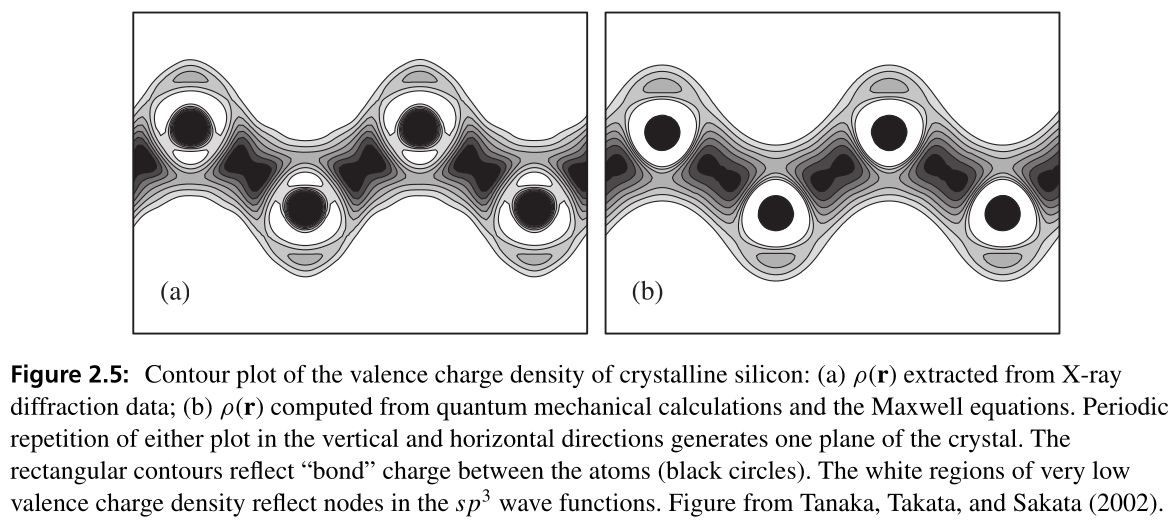
\includegraphics[width=0.7\linewidth]{figura2p5.png}
\end{figure}

\vspace{0.1cm}

\begin{block}{Mensagem final}
O eletromagnetismo clássico vai desde a física de ondas até a estrutura eletrônica da matéria.
\end{block}
\end{frame}

% =========================================================
% 2.3 Microscopic vs Macroscopic
% =========================================================

\section{2.3 Microscópico vs Macroscópico}

% ---------------------------------------------------------
\begin{frame}{2.3 Microscópico vs Macroscópico}
\small

\begin{block}{Ideia de Lorentz}
Hendrik Lorentz percebeu que as equações de Maxwell, formuladas para fenômenos macroscópicos, também são válidas em escala microscópica se \(\rho(\mathbf{r},t)\) e \(\mathbf{j}(\mathbf{r},t)\) forem microscópicos.
\end{block}

\vspace{0.1cm}

\begin{itemize}\setlength{\itemsep}{2pt}
\item Campos microscópicos variam rapidamente no espaço;
\item Medidas macroscópicas capturam apenas médias espaciais;
\item A teoria macroscópica surge de uma média da teoria microscópica.
\end{itemize}

\end{frame}

% ---------------------------------------------------------
\begin{frame}{Validade microscópica}
\footnotesize

\begin{block}{Evidência}
A validade microscópica das equações de Maxwell é confirmada por:
\begin{itemize}\setlength{\itemsep}{2pt}
\item espectro do hidrogênio;
\item concordância teoria-experimento;
\item base da eletrodinâmica quântica (QED).
\end{itemize}
\end{block}

\vspace{0.1cm}

\begin{equation}
E(n,j)=mc^2\left[1+\frac{\alpha^2}{(n-\delta)^2}\right]^{-1/2}
\tag{2.36}
\end{equation}

\begin{equation*}
\delta = j+\frac{1}{2}-\sqrt{\left(j+\frac{1}{2}\right)^2-\alpha^2}
\end{equation*}

\end{frame}

% ---------------------------------------------------------
\begin{frame}{Escalas físicas}
\small

\begin{block}{Mensagem}
As equações de Maxwell são válidas até escalas da ordem do comprimento de Compton:
\[
\lambda_c = \frac{h}{mc}
\]
\end{block}

\vspace{0.1cm}

\begin{itemize}\setlength{\itemsep}{2pt}
\item Não há necessidade de média temporal;
\item Frequências eletrônicas são essenciais (UV, raios X);
\item A média relevante é espacial.
\end{itemize}

\end{frame}

% ---------------------------------------------------------
\subsection{2.3.1 Lorentz Averaging}

\begin{frame}{2.3.1 Média de Lorentz}
\small

\begin{block}{Ideia}
A média espacial transforma grandezas microscópicas em macroscópicas.
\end{block}

\vspace{0.1cm}

Procedimento:
\begin{itemize}\setlength{\itemsep}{2pt}
\item escolher volume \(\Omega\);
\item calcular média espacial;
\item obter campos suaves.
\end{itemize}

\begin{equation}
\mathbf{E}(\mathbf{r},t)
=
\frac{1}{\Omega}\int_\Omega d^3s\,
\mathbf{E}_{\text{micro}}(\mathbf{s}+\mathbf{r},t)
\tag{2.37}
\end{equation}

\end{frame}

% ---------------------------------------------------------
\begin{frame}{Figura de média espacial}
\begin{center}
\begin{figure}
    \centering
    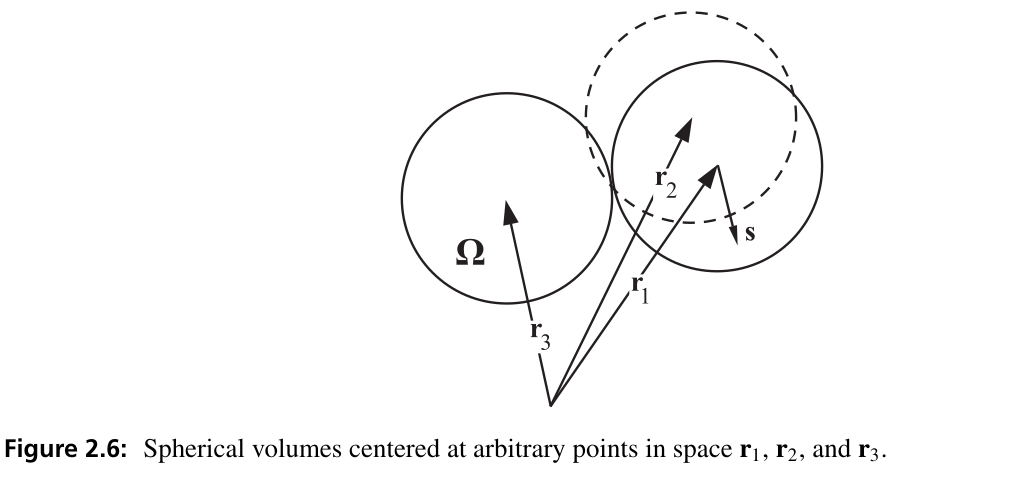
\includegraphics[width=1.0\linewidth]{figure2p6.png}
\end{figure}
\end{center}
\end{frame}

% ---------------------------------------------------------
\begin{frame}{Propriedades da média}
\small

A média de Lorentz é linear e comuta com derivadas:

\begin{equation}
\nabla \times \mathbf{E}(\mathbf{r})
=
\left\langle \nabla \times \mathbf{E}_{\text{micro}} \right\rangle
\tag{2.38}
\end{equation}

\begin{equation}
\frac{\partial \mathbf{E}}{\partial t}
=
\left\langle
\frac{\partial \mathbf{E}_{\text{micro}}}{\partial t}
\right\rangle
\tag{2.39}
\end{equation}

\vspace{0.1cm}

\begin{block}{Conclusão}
As equações de Maxwell têm a mesma forma nas descrições micro e macroscópica.
\end{block}

\end{frame}

% ---------------------------------------------------------
\begin{frame}{Força eletromagnética}
\small

\begin{equation}
\mathbf{F}
=
\int_V d^3r\,
\left[\rho \mathbf{E} + \mathbf{j}\times \mathbf{B}\right]
\tag{2.40}
\end{equation}

\begin{block}{Observação}
A forma da força é mantida ao passar do regime microscópico para o macroscópico.
\end{block}

\end{frame}

% ---------------------------------------------------------
\subsection{2.3.2 Superfície Macroscópica}

\begin{frame}{2.3.2 Superfície macroscópica}
\small

\begin{block}{Problema}
A média espacial gera descontinuidades em superfícies.
\end{block}

\vspace{0.1cm}

\begin{equation}
\bar{\rho}_0(z)
=
\frac{1}{A}\int_A dx\,dy\,\rho_0(\mathbf{r})
\tag{2.41}
\end{equation}

\begin{equation}
\bar{\rho}(z)
=
\bar{\rho}_0(z) + \sigma \lambda(z)
\tag{2.42}
\end{equation}

\end{frame}

% ---------------------------------------------------------
\begin{frame}{Figura de superfície}
\begin{center}
\begin{figure}
    \centering
    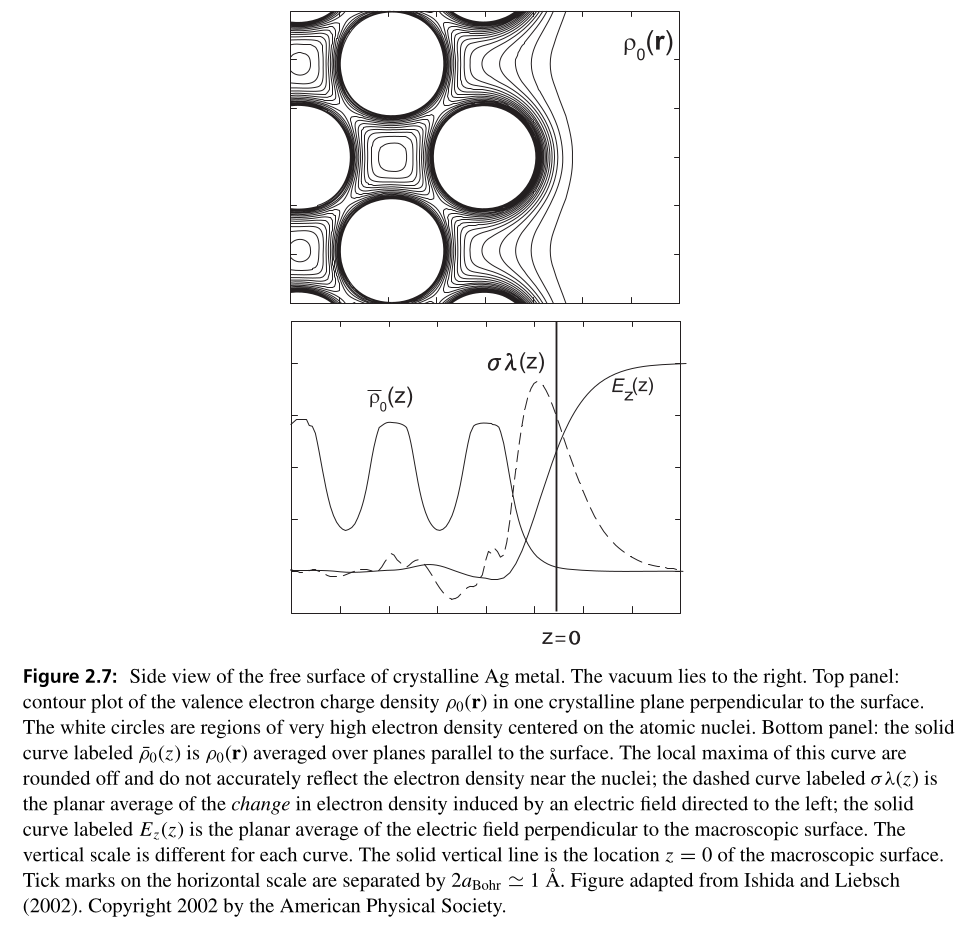
\includegraphics[width=0.5\linewidth]{figura2p7.png}
\end{figure}
\end{center}
\end{frame}

% ---------------------------------------------------------
\begin{frame}{Carga superficial efetiva}
\small

Após média:

\begin{equation}
\sigma \lambda(z) \rightarrow \sigma \delta(z)
\tag{2.43}
\end{equation}

\begin{block}{Interpretação}
A carga microscópica distribuída torna-se uma carga superficial efetiva.
\end{block}

\end{frame}

% ---------------------------------------------------------
% =========================================================
% 2.3.3 Matching Conditions
% =========================================================

\subsection{2.3.3 Condições de contorno (Matching Conditions)}

% ---------------------------------------------------------
\begin{frame}{Interface entre dois meios}
\small

\begin{block}{Situação física}
Considere uma interface plana em \(z=0\), separando dois meios:
\begin{itemize}
\item região \(L\) (esquerda): \(z<0\)
\item região \(R\) (direita): \(z>0\)
\end{itemize}
\end{block}

\vspace{0.1cm}

\begin{itemize}\setlength{\itemsep}{2pt}
\item Campos podem ser diferentes em cada lado:
\[
\mathbf{E}_L(\mathbf{r}), \quad \mathbf{E}_R(\mathbf{r})
\]
\item Pode existir uma \textbf{carga superficial} \(\sigma\) na interface
\end{itemize}

\vspace{0.1cm}

\begin{alertblock}{Pergunta central}
Como os campos elétricos e magnéticos se conectam ao atravessar a interface?
\end{alertblock}

\end{frame}

% ---------------------------------------------------------
\begin{frame}{Ferramenta matemática: função degrau}
\small

Definimos a função degrau:

\begin{equation}
\Theta(z)=
\begin{cases}
0 & z<0 \\
1 & z>0
\end{cases}
\tag{2.44}
\end{equation}

\vspace{0.1cm}

Com isso, escrevemos o campo elétrico como:

\begin{equation}
\mathbf{E}(\mathbf{r})
=
\mathbf{E}_R(\mathbf{r})\,\Theta(z)
+
\mathbf{E}_L(\mathbf{r})\,\Theta(-z)
\tag{2.45}
\end{equation}

\vspace{0.1cm}

\begin{block}{Densidade de carga: similar mas abrimos a possibilidade de haver carga em z=0}
\begin{equation}
\rho(\mathbf{r})
=
\rho_R(\mathbf{r})\,\Theta(z)
+
\rho_L(\mathbf{r})\,\Theta(-z)
+
\sigma\,\delta(z)
\tag{2.46}
\end{equation}
\end{block}

\end{frame}

% ---------------------------------------------------------
\begin{frame}{Passo chave: divergência}
\small

Aplicamos a lei de Gauss:

\[
\nabla\cdot \mathbf{E} = \frac{\rho}{\epsilon_0}
\]

\vspace{0.1cm}

Tomando a divergência de \(\mathbf{E}\):

\begin{equation}
\nabla\cdot \mathbf{E}
=
[\nabla\cdot \mathbf{E}_R]\Theta(z)
+
[\nabla\cdot \mathbf{E}_L]\Theta(-z)
+
\hat{\mathbf{z}}\cdot(\mathbf{E}_R-\mathbf{E}_L)\,\delta(z)
\tag{2.47}
\end{equation}

\vspace{0.1cm}

\begin{block}{Ideia importante}
A derivada da função degrau gera uma \textbf{delta de Dirac}, responsável pelo termo de descontinuidade.
\end{block}

\end{frame}

% ---------------------------------------------------------
\begin{frame}{Resultado principal}
\small

Comparando com a expressão da densidade de carga:

\[
\rho(\mathbf{r}) = \rho_R\Theta(z)+\rho_L\Theta(-z)+\sigma\delta(z)
\]

obtemos:

\begin{equation}
\hat{\mathbf{z}}\cdot(\mathbf{E}_R-\mathbf{E}_L)
=
\frac{\sigma}{\epsilon_0}
\tag{2.48}
\end{equation}

Esta é uma condição de compatibilidade que relaciona a descontinuidade na componente normal do campo elétrico macroscópico à magnitude da densidade de carga singular na interface.

\vspace{0.2cm}

\begin{alertblock}{Interpretação física}
\begin{itemize}
\item O campo elétrico sofre um \textbf{salto na direção normal}
\item Esse salto é proporcional à \textbf{carga superficial}
\end{itemize}
\end{alertblock}

\end{frame}

\begin{frame}{Condição de contorno do campo elétrico}

\begin{block}{Interpretação física}
Se existir carga acumulada na interface (em \(z = 0\)), então o campo elétrico não pode ser contínuo ali — ele sofre um “salto” na componente perpendicular à superfície.
\end{block}

\vspace{0.2cm}

\begin{itemize}
\item A componente \textbf{normal} do campo elétrico (perpendicular à superfície) muda ao atravessar a interface.
\item O tamanho dessa mudança é proporcional à densidade de carga superficial \(\sigma\).
\end{itemize}

\vspace{0.3cm}

\begin{alertblock}{Condição de contorno}
\begin{equation}
E_{\perp}^{\text{acima}} - E_{\perp}^{\text{abaixo}} = \frac{\sigma}{\epsilon_0}
\label{eq:condicao_contorno_E}
\end{equation}
\end{alertblock}

\end{frame}
% ---------------------------------------------------------
\begin{frame}{Visualização da interface}
\begin{center}
\fbox{
\begin{minipage}[c][0.55\textheight][c]{0.85\textwidth}
\centering
\begin{figure}
    \centering
    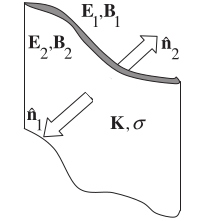
\includegraphics[width=0.3\linewidth]{figura2p8.png}
\end{figure}
\end{minipage}
}
\end{center}

\vspace{0.1cm}

\small
\centering Interface com densidade de carga \(\sigma\) e corrente superficial \(\mathbf{K}\)

\end{frame}

% ---------------------------------------------------------
\begin{frame}{Condições gerais de contorno}
\small

Para uma interface com \(\sigma\) e corrente superficial \(\mathbf{K}\):

\vspace{0.1cm}

\begin{block}{Componentes normais}
\begin{equation*}
\hat{\mathbf{n}}\cdot(\mathbf{E}_1-\mathbf{E}_2)=\frac{\sigma}{\epsilon_0}
\end{equation*}

\begin{equation*}
\hat{\mathbf{n}}\cdot(\mathbf{B}_1-\mathbf{B}_2)=0
\end{equation*}
\end{block}

\vspace{0.1cm}

\begin{block}{Componentes tangenciais}
\begin{equation*}
\hat{\mathbf{n}}\times(\mathbf{E}_1-\mathbf{E}_2)=0
\end{equation*}

\begin{equation}
\hat{\mathbf{n}}\times(\mathbf{B}_1-\mathbf{B}_2)=\mu_0 \mathbf{K}
\tag{2.49}
\end{equation}
\end{block}

\end{frame}

% ---------------------------------------------------------
\begin{frame}{Interpretação física}
\small

\begin{itemize}\setlength{\itemsep}{3pt}
\item \(\mathbf{E}_\perp\) é descontínuo → devido a \(\sigma\)
\item \(\mathbf{B}_\perp\) é contínuo → não há monopolos magnéticos
\item \(\mathbf{E}_\parallel\) é contínuo → lei de Faraday
\item \(\mathbf{B}_\parallel\) é descontínuo → devido a corrente \(\mathbf{K}\)
\end{itemize}

\vspace{0.2cm}

\begin{alertblock}{Mensagem central}
As condições de contorno são uma consequência direta das equações de Maxwell aplicadas a interfaces.
\end{alertblock}

\end{frame}

% ---------------------------------------------------------
\begin{frame}{Interface em movimento}
\small

Se a interface se move com velocidade \(\mathbf{v}\):

\begin{equation}
\hat{\mathbf{n}} \times (\mathbf{E}_1-\mathbf{E}_2)
-
(\mathbf{v}\cdot \hat{\mathbf{n}})(\mathbf{B}_1-\mathbf{B}_2)
=0
\tag{2.50}
\end{equation}

\begin{equation}
\hat{\mathbf{n}} \times (\mathbf{B}_1-\mathbf{B}_2)
+
\frac{\mathbf{v}\cdot \hat{\mathbf{n}}}{c^2}
(\mathbf{E}_1-\mathbf{E}_2)
=
\mu_0 \mathbf{K}
\end{equation}

\vspace{0.1cm}

\begin{block}{Observação}
Essas correções aparecem por efeitos relativísticos.
\end{block}

\end{frame}


%====================================================
\begin{frame}{Problema 2.3 - Zangwill pag 55}

\begin{block}{Enunciado}
Sejam \(\mathbf{r}_1\) e \(\mathbf{r}_2\) vetores que apontam para elementos de linha \(d\mathbf{s}_1\) e \(d\mathbf{s}_2\) de duas espiras fechadas \(C_1\) e \(C_2\), percorridas por correntes \(I_1\) e \(I_2\), respectivamente. Experimentalmente, a força exercida sobre \(I_1\) por \(I_2\) é
\begin{equation}
\mathbf{F}_1
=
-\frac{\mu_0}{4\pi}
\oint_{C_1} I_1\,d\mathbf{s}_1 \cdot
\oint_{C_2} I_2\,d\mathbf{s}_2\,
\frac{\mathbf{r}_1-\mathbf{r}_2}{|\mathbf{r}_1-\mathbf{r}_2|^3}.
\label{eq:p23_forca_inicial}
\end{equation}

Mostre que:
\begin{enumerate}
\item[(a)]
\begin{equation}
\oint_{C_1}
d\mathbf{s}_1 \cdot
\frac{\mathbf{r}_1-\mathbf{r}_2}{|\mathbf{r}_1-\mathbf{r}_2|^3}
=0.
\label{eq:p23_item_a}
\end{equation}

\item[(b)] Usando (a), mostre que
\begin{equation}
\mathbf{F}_1
=
\oint_{C_1}
I_1\,d\mathbf{s}_1 \times \mathbf{B}_2(\mathbf{r}_1),
\label{eq:p23_item_b}
\end{equation}
onde \(\mathbf{B}_2(\mathbf{r})\) é o campo magnético produzido pela espira \(C_2\).
\end{enumerate}
\end{block}
\notas{pag 12-21}
\end{frame}

\begin{frame}{Problema 2.11 - Zangwill pag 56}

\begin{block}{Enunciado}
Uma densidade de corrente superficial \(\mathbf{K}(\mathbf{r}_s,t)\) flui no plano \(z=0\), separando a região 1 (\(z>0\)) da região 2 (\(z<0\)). Cada região contém distribuições arbitrárias e dependentes do tempo de carga e corrente.

\medskip

(a) Para os campos \(\mathbf{B}(\mathbf{r},t)\) e \(\mathbf{E}(\mathbf{r},t)\), use o método da função degrau para derivar uma condição de contorno a partir da lei de Ampère--Maxwell:
\begin{equation}
\nabla \times \mathbf{B}
=
\mu_0 \mathbf{j}
+
\frac{1}{c^2}\frac{\partial \mathbf{E}}{\partial t}.
\label{eq:ampere_maxwell}
\end{equation}

(b) Explique como adaptar o resultado para uma interface não plana.
\end{block}

\notas{pag 22-28}
\end{frame}


\begin{frame}{Interpretação física}

\begin{itemize}
\item Apenas a componente \textbf{tangencial} de \(\mathbf{B}\) é descontínua
\item A descontinuidade é proporcional à corrente superficial
\item Campo magnético “gira” ao redor da corrente (regra da mão direita)
\end{itemize}

\begin{block}{Forma equivalente}
\begin{equation}
\mathbf{B}_1 - \mathbf{B}_2
=
\mu_0\, \mathbf{K} \times \hat{\mathbf{n}}
\end{equation}
\end{block}

\end{frame}

%====================================================
\begin{frame}{Parte (b) --- Interface não plana}

\begin{block}{Generalização}
Para uma superfície arbitrária:

\begin{equation}
\hat{\mathbf{n}}(\mathbf{r}_s) \times (\mathbf{B}_1 - \mathbf{B}_2)
=
\mu_0 \mathbf{K}(\mathbf{r}_s)
\label{eq:geral}
\end{equation}

\end{block}

\begin{itemize}
\item \(\hat{\mathbf{n}}\) é o vetor normal local
\item A condição é válida ponto a ponto
\item A curvatura da superfície não altera a estrutura da equação
\end{itemize}

\end{frame}



%====================================================
\section{2.4 As Equações de Maxwell na Matéria}


\begin{frame}[plain]
\begin{center}

\vspace{1cm}

{\Huge \textbf{\blue{2.4}}}

\vspace{0.5cm}

{\LARGE \textbf{Equações de Maxwell na Matéria}}

\vspace{1.5cm}

{\large Eletrodinâmica Clássica}


\end{center}
\end{frame}


\begin{frame}{O problema físico: por que complicar Maxwell?}

\begin{block}{Situação inicial}
Até agora, tratamos:
\[
\rho,\ \mathbf{j} \quad \Rightarrow \quad \mathbf{E},\ \mathbf{B}
\]
como se tudo fosse \textbf{vácuo}.
\end{block}

\pause

\begin{block}{Mas na prática...}
\begin{itemize}
\item Quase tudo ocorre em \textbf{materiais}
\item A matéria responde aos campos:
\begin{itemize}
\item desloca cargas
\item cria correntes internas
\end{itemize}
\end{itemize}
\end{block}

\end{frame}

\begin{frame}[plain]

\begin{alertblock}{Problema}
Como separar:
\begin{itemize}
\item o que é \textbf{fonte externa}
\item do que é \textbf{resposta da matéria}?
\end{itemize}
\end{alertblock}

\end{frame}

%====================================================

\begin{frame}{A solução de Maxwell}

\begin{block}{Ideia genial}
Separar as fontes em:
\begin{itemize}
\item \textbf{livres} (controladas externamente)
\item \textbf{ligadas} (resposta da matéria)
\end{itemize}
\end{block}

\pause

\begin{block}{Consequência}
Precisamos de novos campos:
\[
\mathbf{D}, \quad \mathbf{H}
\]
\end{block}

\pause

\begin{alertblock}{Mensagem física}
\[
\mathbf{E}, \mathbf{B} \Rightarrow \text{campos físicos}
\]
\[
\mathbf{D}, \mathbf{H} \Rightarrow \text{organizam a matéria}
\]
\end{alertblock}

\end{frame}

%====================================================

\section{Fontes dentro da matéria}

\begin{frame}{O que a matéria faz?}

\begin{block}{Resposta microscópica}
Quando aplicamos um campo:
\begin{itemize}
\item elétrons se deslocam
\item dipolos se alinham
\item correntes microscópicas aparecem
\end{itemize}
\end{block}

\pause

\begin{block}{Modelagem macroscópica}
Introduzimos:

\[
\mathbf{P}(\mathbf{r},t) \quad \text{(polarização)}
\]
\[
\mathbf{M}(\mathbf{r},t) \quad \text{(magnetização)}
\]

\end{block}

\end{frame}

%====================================================

\begin{frame}{Como isso vira carga e corrente?}

\begin{block}{Carga total}
\begin{equation}
\rho = \rho_f - \nabla \cdot \mathbf{P}
\end{equation}
\end{block}

\pause

\begin{block}{Corrente total}
\begin{equation}
\mathbf{j} =
\mathbf{j}_f
+
\nabla \times \mathbf{M}
+
\frac{\partial \mathbf{P}}{\partial t}
\end{equation}
\end{block}

\pause

\begin{alertblock}{Interpretação}
\begin{itemize}
\item \(-\nabla\cdot\mathbf{P}\): cargas ligadas
\item \(\nabla\times\mathbf{M}\): correntes internas
\item \(\partial_t \mathbf{P}\): deslocamento de cargas
\end{itemize}
\end{alertblock}

\end{frame}

%====================================================

\section{Campos auxiliares}

\begin{frame}{Definição de \(\mathbf{D}\) e \(\mathbf{H}\)}

\begin{block}{Campos auxiliares}
\begin{equation}
\mathbf{D} = \epsilon_0 \mathbf{E} + \mathbf{P}
\end{equation}

\begin{equation}
\mathbf{H} = \frac{1}{\mu_0}\mathbf{B} - \mathbf{M}
\end{equation}
\end{block}

\pause

\begin{alertblock}{Por quê?}
Essas definições:
\begin{itemize}
\item absorvem a resposta da matéria
\item deixam apenas fontes livres nas equações
\end{itemize}
\end{alertblock}

\end{frame}

%====================================================

\begin{frame}{Maxwell reorganizado}

\begin{block}{Forma elegante}
\begin{equation}
\nabla \cdot \mathbf{D} = \rho_f
\end{equation}

\begin{equation}
\nabla \times \mathbf{H} =
\mathbf{j}_f + \frac{\partial \mathbf{D}}{\partial t}
\end{equation}
\end{block}

\pause

\begin{block}{O que mudou?}
\begin{itemize}
\item Só aparecem fontes \textbf{livres}
\item Toda a complexidade da matéria foi escondida em:
\[
\mathbf{D}, \mathbf{H}
\]
\end{itemize}
\end{block}

\end{frame}

%====================================================

\section{Condições de contorno}

\begin{frame}{O que acontece na interface?}

\begin{block}{Situação física}
Dois materiais diferentes em contato
\end{block}

\pause

\begin{block}{Pergunta}
Como os campos mudam ao atravessar a interface?
\end{block}

\end{frame}

%====================================================

\begin{frame}{Resultados fundamentais}

\begin{block}{Campos elétricos}
\begin{equation}
\hat{\mathbf n}\cdot(\mathbf{D}_1-\mathbf{D}_2)=\sigma_f
\end{equation}
\end{block}

\pause

\begin{block}{Campos magnéticos}
\begin{equation}
\hat{\mathbf n}\times(\mathbf{H}_1-\mathbf{H}_2)=\mathbf{K}_f
\end{equation}
\end{block}

\pause

\begin{alertblock}{Leitura física}
\begin{itemize}
\item cargas livres quebram a componente normal de \(\mathbf D\)
\item correntes livres quebram a componente tangencial de \(\mathbf H\)
\end{itemize}
\end{alertblock}

\end{frame}

%====================================================

\section{Exemplo físico}

\begin{frame}{Exemplo: capacitor com dielétrico}

\begin{block}{Situação}
\begin{itemize}
\item placas com carga livre
\item material polarizável no meio
\end{itemize}
\end{block}

\pause

\begin{block}{O que acontece?}
\begin{itemize}
\item \(\mathbf{E}\) diminui dentro do material
\item \(\mathbf{P}\) aparece
\item \(\mathbf{D}\) continua ligado à carga livre
\end{itemize}
\end{block}

\pause

\begin{alertblock}{Mensagem}
\[
\mathbf{D} \text{ "vê" apenas as cargas livres}
\]
\end{alertblock}

\end{frame}

%====================================================

\section{Relações constitutivas}

\begin{frame}{Como fechar o sistema?}

\begin{block}{Problema}
Maxwell não diz como a matéria responde.
\end{block}

\pause

\begin{block}{Solução}
Relações constitutivas:
\begin{equation}
\mathbf{D}=\epsilon \mathbf{E}, \quad
\mathbf{B}=\mu \mathbf{H}
\end{equation}
\end{block}

\pause

\begin{alertblock}{Importante}
\begin{itemize}
\item válidas para materiais simples
\item aproximação linear
\end{itemize}
\end{alertblock}

\end{frame}

%====================================================

\section{Mensagem final}

\begin{frame}{O que você deve guardar}

\begin{alertblock}{Ideia central do capítulo}
\begin{itemize}
\item A matéria não cria novas leis
\item Ela modifica como as fontes aparecem
\end{itemize}
\end{alertblock}

\pause

\begin{block}{Resumo mental}
\begin{itemize}
\item \(\mathbf{E}, \mathbf{B}\): campos físicos reais
\item \(\mathbf{D}, \mathbf{H}\): reorganizam o problema
\item \(\mathbf{P}, \mathbf{M}\): resposta da matéria
\end{itemize}
\end{block}




\end{frame}


\begin{frame}{Exemplo aplicado: capacitor com dielétrico linear}

\begin{block}{Situação física}
Considere um capacitor de placas paralelas, totalmente preenchido por um dielétrico linear, homogêneo e isotrópico, de permissividade
\[
\epsilon = \epsilon_0(1+\chi_e)=\epsilon_r\epsilon_0.
\]
As placas têm densidades superficiais de carga livre \(+\sigma_f\) e \(-\sigma_f\).
\end{block}

\end{frame}


\begin{frame}{Capacitor com dielétrico}
\begin{figure}
    \centering
    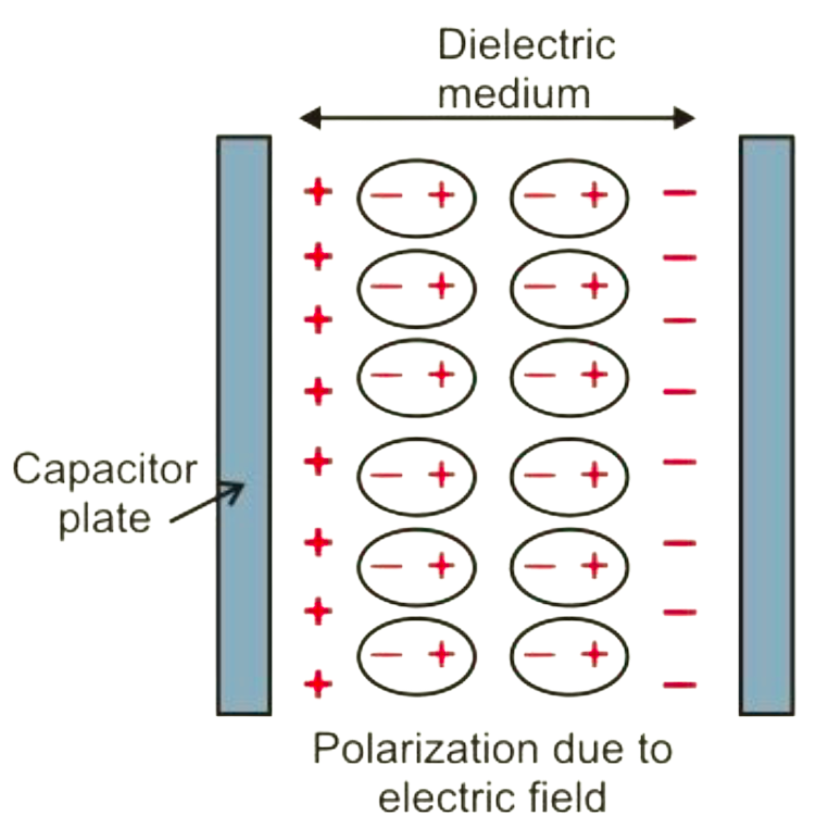
\includegraphics[width=0.5\linewidth]{capacitor.png}

\end{figure}
    
\end{frame}

\begin{frame}{Susceptibilidade elétrica \(\chi_e\)}

\begin{block}{O que ela representa}
É uma medida de quanto o material se polariza quando submetido a um campo elétrico:
\begin{equation}
\mathbf{P} = \epsilon_0 \chi_e \mathbf{E}
\label{eq:susc_def}
\end{equation}
\end{block}

\vspace{0.2cm}

\begin{block}{Interpretação física}
\begin{itemize}
\item \(\chi_e = 0\) \quad $\rightarrow$ vácuo (não há resposta)
\item \(\chi_e > 0\) \quad $\rightarrow$ material se polariza na direção do campo
\item \(\chi_e \gg 1\) \quad $\rightarrow$ material muito polarizável
\end{itemize}
\end{block}

\vspace{0.2cm}

\begin{alertblock}{Relação importante}
Ela está ligada à permissividade:
\begin{equation}
\epsilon = \epsilon_0 (1 + \chi_e)
\label{eq:epsilon_chi}
\end{equation}
\end{alertblock}

\end{frame}

\begin{frame}

\vspace{0.2cm}

\begin{block}{Passo 1: campo \(\mathbf{D}\)}
Pela lei de Gauss na matéria,
\begin{equation}
\nabla\cdot\mathbf{D}=\rho_f.
\end{equation}

Para essa geometria,
\begin{equation}
\mathbf{D}=\sigma_f\,\hat{\mathbf{n}},
\end{equation}
apontando da placa positiva para a negativa.
\end{block}

\end{frame}

%--------------------------------------------------

\begin{frame}{Exemplo aplicado: obtendo \(\mathbf{E}\), \(\mathbf{P}\) e cargas ligadas}

\begin{block}{Passo 2: campo elétrico}
Como o meio é linear,
\begin{equation}
\mathbf{D}=\epsilon \mathbf{E}.
\end{equation}

Logo,
\begin{equation}
\mathbf{E}=\frac{\mathbf{D}}{\epsilon}
=\frac{\sigma_f}{\epsilon}\,\hat{\mathbf{n}}.
\end{equation}
\end{block}

\pause

\begin{block}{Passo 3: polarização}
Usando
\begin{equation}
\mathbf{P}=\epsilon_0\chi_e \mathbf{E},
\end{equation}
obtemos
\begin{equation}
\mathbf{P}
=
\epsilon_0\chi_e\frac{\sigma_f}{\epsilon}\,\hat{\mathbf{n}}
=
\frac{\chi_e}{1+\chi_e}\,\sigma_f\,\hat{\mathbf{n}}.
\end{equation}
\end{block}


\end{frame}


\begin{frame}

\begin{alertblock}{Cargas ligadas}
No volume,
\begin{equation}
\rho_b=-\nabla\cdot \mathbf{P}=0
\end{equation}
(pois \(\mathbf{P}\) é uniforme), enquanto nas superfícies do dielétrico:
\begin{equation}
\sigma_b=\mathbf{P}\cdot \hat{\mathbf{n}}.
\end{equation}
\end{alertblock}

\end{frame}

%--------------------------------------------------

\begin{frame}{Leitura física do exemplo}

\begin{block}{Resultado final}
\begin{equation}
\mathbf{D}=\sigma_f\,\hat{\mathbf{n}},
\qquad
\mathbf{E}=\frac{\sigma_f}{\epsilon}\,\hat{\mathbf{n}},
\qquad
\mathbf{P}=\epsilon_0\chi_e\mathbf{E}.
\end{equation}
\end{block}

\pause

\begin{itemize}
\item \(\mathbf{D}\) é determinado apenas pela \textbf{carga livre}.
\item \(\mathbf{E}\) fica \textbf{reduzido} pelo dielétrico.
\item A matéria responde criando \textbf{cargas ligadas} nas superfícies.
\end{itemize}

\pause

\begin{alertblock}{Mensagem física}
O formalismo de \(\mathbf{D}\) e \(\mathbf{P}\) separa claramente:
\[
\text{fonte externa} \quad \text{vs} \quad \text{resposta da matéria}.
\]
\end{alertblock}

\end{frame}


%====================================================
\section{Polarização do Vácuo}

\begin{frame}{2.5.2 Polarização do Vácuo}

\begin{block}{Ideia surpreendente}
Mesmo o \textbf{vácuo} pode se comportar como um meio material.
\end{block}

\pause

\begin{alertblock}{Por quê?}
Na eletrodinâmica quântica (QED):
\begin{itemize}
\item o vácuo não é "vazio"
\item existem flutuações quânticas
\item pares elétron–pósitron aparecem virtualmente
\end{itemize}
\end{alertblock}

\end{frame}

\begin{frame}[plain]

\begin{block}{Consequência}
O vácuo pode:
\begin{itemize}
\item se polarizar
\item modificar campos elétricos
\item introduzir não linearidades em Maxwell
\end{itemize}
\end{block}

\end{frame}

%====================================================

\begin{frame}{Analogia com dielétricos}

\begin{block}{Em materiais}
\[
\mathbf{P} = \epsilon_0 \chi_e \mathbf{E}
\]
\end{block}

\pause

\begin{block}{No vácuo quântico}
\begin{itemize}
\item o campo elétrico cria pares virtuais
\item esses pares se alinham → polarização do vácuo
\end{itemize}
\end{block}

\pause

\begin{alertblock}{Interpretação}
\[
\text{O vácuo funciona como um dielétrico extremamente fraco}
\]
\end{alertblock}

\end{frame}

%====================================================

\begin{frame}{Correção ao potencial de Coulomb}

\begin{block}{Resultado da QED}
O potencial de uma carga não é exatamente:
\[
\phi(r) = \frac{q}{4\pi\epsilon_0 r}
\]
\end{block}

\pause

\begin{block}{Correção (curtas distâncias)}
\begin{equation}
\phi(r)
\sim
\frac{q}{4\pi\epsilon_0 r}
\left[
1 - \frac{2\alpha}{3\pi}\ln\left(\frac{r}{\lambda_c}\right)
\right]
\end{equation}
\end{block}
$\text{onde } q \text{ é a carga elétrica, } \epsilon_0 \text{ é a permissividade do vácuo, } 

\alpha \text{ é a constante de estrutura fina, } r \text{ é a distância ao ponto de carga, e }

\lambda_c \text{ é o comprimento de Compton da partícula.}$


\end{frame}

\begin{frame}
\begin{alertblock}{Interpretação}
\begin{itemize}
\item a carga "efetiva" depende da escala
\item fenômeno de \textbf{renormalização}
\end{itemize}
\end{alertblock}

\end{frame}

%====================================================

\begin{frame}{Ideia profunda: carga depende da escala}

\begin{block}{O que está acontecendo?}
\begin{itemize}
\item perto da carga → vácuo altamente polarizado
\item longe → efeito diminui
\end{itemize}
\end{block}

\pause

\begin{alertblock}{Conclusão}
\[
q_{\text{efetiva}} = q(r)
\]
\end{alertblock}

\pause

\begin{block}{Conexão moderna}
Isso é a base de:
\begin{itemize}
\item teoria de renormalização
\item grupo de renormalização
\item física de partículas moderna
\end{itemize}
\end{block}

\end{frame}

%====================================================

\begin{frame}{Quando o efeito fica importante?}

\begin{block}{Campo crítico de Schwinger}
\begin{equation}
E_c \sim \frac{m_e^2 c^3}{e\hbar} \sim 10^{18}\ \text{V/m}
\end{equation}
\end{block}

\pause

\begin{block}{Campo magnético crítico}
\begin{equation}
B_c \sim 10^9\ \text{T} \;\; \approx \;\; 10^{13}\ \text{G}
\end{equation}
\end{block}

\pause

\begin{alertblock}{Comparação}
\begin{itemize}
\item Laboratório: até \(10^6\ \text{V/m}\)
\item Estrelas de nêutrons: \(10^{9} - 10^{11}\ \text{T} \;\; \approx \;\; 10^{13} - 10^{15}\ \text{G}\)
\end{itemize}
\end{alertblock}
\end{frame}

%====================================================

\begin{frame}{Exemplo astrofísico: magnetars}

\begin{block}{Magnetars}
\begin{itemize}
\item estrelas de nêutrons altamente magnetizadas
\item campos até:
\[
B \sim 10^{11}\ \text{T} =  \;\;  10^{15}\ \text{G}
\]
\end{itemize}
\end{block}

\pause

\begin{alertblock}{Consequência}
\begin{itemize}
\item vácuo se torna \textbf{birrefringente}
\item luz se propaga como em um cristal
\end{itemize}
\end{alertblock}

\pause

\begin{block}{Observação real}
Polarização da luz observada em:
\begin{itemize}
\item RX J1856.5–3754 (ESO, 2017)
\end{itemize}
\end{block}

\end{frame}

%====================================================

\begin{frame}{Eletrodinâmica não linear}

\begin{block}{Resultado de QED}
Campos fortes geram:
\begin{equation}
\mathbf{P} \sim (E^2 - c^2 B^2)\mathbf{E}
\end{equation}
\end{block}

\pause

\begin{block}{Consequência}
\begin{itemize}
\item princípio da superposição quebra
\item Maxwell deixa de ser linear
\end{itemize}
\end{block}

\pause

\begin{alertblock}{Nome}
Eletrodinâmica de Euler–Heisenberg
\end{alertblock}

\end{frame}

%====================================================

\begin{frame}{Experimentos atuais}

\begin{block}{Laboratórios modernos}
\begin{itemize}
\item lasers ultra intensos (ELI, XFEL)
\item colisões de fótons
\end{itemize}
\end{block}

\pause

\begin{block}{O que se busca}
\begin{itemize}
\item produção de pares
\item espalhamento fóton–fóton
\item birefringência do vácuo
\end{itemize}
\end{block}

\pause

\begin{alertblock}{Paper recente}
\begin{itemize}
\item ATLAS Collaboration (2017): evidência de light-by-light scattering
\end{itemize}
\end{alertblock}

\end{frame}

%====================================================

\begin{frame}{Resumo conceitual}

\begin{alertblock}{Mensagem principal}
\begin{itemize}
\item o vácuo não é vazio
\item ele responde a campos → polarização
\item isso modifica a física clássica
\end{itemize}
\end{alertblock}

\pause

\begin{block}{Conexões}
\begin{itemize}
\item QED
\item astrofísica relativística
\item lasers ultra intensos
\end{itemize}
\end{block}



\end{frame}



%====================================================
%====================================================
\begin{frame}{Exercício aplicado: capacitor com dielétrico}

\begin{block}{Situação física}
Um capacitor de placas paralelas, com área
\[
A = 2,0\times 10^{-2}\ \text{m}^2
\]
e separação
\[
d = 1,0\times 10^{-3}\ \text{m},
\]
é totalmente preenchido por um dielétrico linear, homogêneo e isotrópico com susceptibilidade elétrica
\[
\chi_e = 4.
\]

As placas possuem cargas livres \(\pm Q_f\), com
\[
Q_f = 1,0\times 10^{-8}\ \text{C}.
\]
\end{block}

\end{frame}

%====================================================

\begin{frame}{Exercício aplicado: capacitor com dielétrico}

\begin{block}{Dados}
Adote:
\[
\epsilon_0 = 8{,}85\times 10^{-12}\ \text{F/m}.
\]
\end{block}

\begin{alertblock}{Pede-se}
Determinar:
\begin{enumerate}
\item a densidade de carga livre \(\sigma_f\);
\item o campo deslocamento \(\mathbf D\);
\item o campo elétrico \(\mathbf E\);
\item a polarização \(\mathbf P\);
\item a densidade de carga ligada superficial \(\sigma_b\);
\item a diferença de potencial entre as placas.
\end{enumerate}
\end{alertblock}

\end{frame}

%====================================================

\begin{frame}{Resolução: passo 1 --- densidade de carga livre}

A densidade de carga livre nas placas é

\begin{equation}
\sigma_f = \frac{Q_f}{A}.
\end{equation}

Substituindo os valores:

\begin{equation}
\sigma_f
=
\frac{1,0\times 10^{-8}}{2,0\times 10^{-2}}
=
5,0\times 10^{-7}\ \text{C/m}^2.
\end{equation}

\begin{alertblock}{Resultado}
\begin{equation}
\sigma_f = 5,0\times 10^{-7}\ \text{C/m}^2
\end{equation}
\end{alertblock}

\end{frame}

%====================================================

\begin{frame}{Resolução: passo 2 --- campo \(\mathbf D\)}

Para um capacitor plano totalmente preenchido por dielétrico, vale

\begin{equation}
\mathbf D = \sigma_f \,\hat{\mathbf n},
\end{equation}
onde \(\hat{\mathbf n}\) aponta da placa positiva para a negativa.

Portanto,

\begin{equation}
\mathbf D = 5,0\times 10^{-7}\,\hat{\mathbf n}\ \text{C/m}^2.
\end{equation}

\begin{alertblock}{Resultado}
\begin{equation}
|\mathbf D| = 5,0\times 10^{-7}\ \text{C/m}^2
\end{equation}
\end{alertblock}

\begin{block}{Interpretação}
O campo \(\mathbf D\) depende apenas da carga \textbf{livre}.
\end{block}

\end{frame}

%====================================================

\begin{frame}{Resolução: passo 3 --- campo elétrico \(\mathbf E\)}

Como o meio é linear,

\begin{equation}
\mathbf D = \epsilon \mathbf E,
\end{equation}
com
\begin{equation}
\epsilon = \epsilon_0(1+\chi_e).
\end{equation}

Como \(\chi_e=4\),

\begin{equation}
\epsilon = 5\epsilon_0.
\end{equation}

Logo,

\begin{equation}
E=\frac{D}{\epsilon}
=
\frac{5,0\times 10^{-7}}{5\times 8{,}85\times 10^{-12}}.
\end{equation}

\begin{equation}
E \approx 1{,}13\times 10^4\ \text{V/m}.
\end{equation}

\begin{alertblock}{Resultado}
\begin{equation}
\mathbf E \approx 1{,}13\times 10^4\,\hat{\mathbf n}\ \text{V/m}
\end{equation}
\end{alertblock}

\end{frame}

%====================================================

\begin{frame}{Resolução: passo 4 --- polarização \(\mathbf P\)}

A polarização vale

\begin{equation}
\mathbf P = \epsilon_0 \chi_e \mathbf E.
\end{equation}

Substituindo:

\begin{equation}
P
=
(8{,}85\times 10^{-12})(4)(1{,}13\times 10^4).
\end{equation}

\begin{equation}
P \approx 4{,}0\times 10^{-7}\ \text{C/m}^2.
\end{equation}

\begin{alertblock}{Resultado}
\begin{equation}
\mathbf P \approx 4{,}0\times 10^{-7}\,\hat{\mathbf n}\ \text{C/m}^2
\end{equation}
\end{alertblock}

\begin{block}{Leitura física}
O dielétrico se polariza na direção do campo, reduzindo o campo elétrico interno.
\end{block}

\end{frame}

%====================================================

\begin{frame}{Resolução: passo 5 --- carga ligada superficial}

Como \(\mathbf P\) é uniforme no interior, temos

\begin{equation}
\rho_b = -\nabla\cdot \mathbf P = 0.
\end{equation}

Mas surgem cargas ligadas nas superfícies do dielétrico, com densidade

\begin{equation}
\sigma_b = \mathbf P \cdot \hat{\mathbf n}.
\end{equation}

Assim, em módulo,

\begin{equation}
\sigma_b = P \approx 4{,}0\times 10^{-7}\ \text{C/m}^2.
\end{equation}

\begin{alertblock}{Resultado}
\begin{equation}
|\sigma_b| \approx 4{,}0\times 10^{-7}\ \text{C/m}^2
\end{equation}
\end{alertblock}

\end{frame}

\begin{frame}

\begin{block}{Observação}
As cargas ligadas têm sinais opostos nas duas faces do dielétrico.
\end{block}

\end{frame}

%====================================================

\begin{frame}{Resolução: passo 6 --- diferença de potencial}

Para campo uniforme,

\begin{equation}
V = Ed.
\end{equation}

Logo,

\begin{equation}
V = (1{,}13\times 10^4)(1{,}0\times 10^{-3})
\approx 11{,}3\ \text{V}.
\end{equation}

\begin{alertblock}{Resultado}
\begin{equation}
V \approx 11{,}3\ \text{V}
\end{equation}
\end{alertblock}

\end{frame}

%====================================================

\begin{frame}{Resumo final do exercício}

\begin{block}{Resultados}
\begin{align}
\sigma_f &= 5,0\times 10^{-7}\ \text{C/m}^2 \\
D &= 5,0\times 10^{-7}\ \text{C/m}^2 \\
E &\approx 1{,}13\times 10^4\ \text{V/m} \\
P &\approx 4,0\times 10^{-7}\ \text{C/m}^2 \\
|\sigma_b| &\approx 4,0\times 10^{-7}\ \text{C/m}^2 \\
V &\approx 11,3\ \text{V}
\end{align}
\end{block}

\end{frame}


\begin{frame}

\begin{alertblock}{Mensagem física}
\begin{itemize}
\item \(\mathbf D\) é controlado pela carga livre
\item o dielétrico cria polarização \(\mathbf P\)
\item essa polarização reduz o campo \(\mathbf E\)
\item surgem cargas ligadas nas superfícies do material
\end{itemize}
\end{alertblock}

\end{frame}



\end{document}
